% =====================================================================================
% Fashion-MNIST Classical ML Benchmark: Capstone Phase 1 report (IEEE conference format)
%
% HOW TO COMPILE (e.g. Overleaf):
%   1. Create a new project and paste this file as main.tex.
%   2. Create a folder "figures/" and upload these PNGs from results/figures/ in the repo:
%        eda_class_mean_images.png   eda_tsne.png               features_hog_examples.png
%        results_pixels_vs_hog.png   results_acc_vs_time.png    results_recall_heatmap.png
%        errors_confusion_rbf_svm_hog.png   errors_misclassified_shirt_vs_t-shirt_top.png
%   3. Compile with pdfLaTeX. IEEEtran is built into Overleaf.
%   4. Fill in the TODO lines (university / department / course).
% Every number below comes from results/summary.csv and results/metrics/*.json in the repo.
% =====================================================================================
\documentclass[conference]{IEEEtran}
\usepackage[utf8]{inputenc}
\usepackage[T1]{fontenc}
\usepackage{graphicx}
\usepackage{booktabs}
\usepackage{amsmath}
\usepackage{url}
\usepackage{cite}
\usepackage[hidelinks]{hyperref}
\graphicspath{{figures/}}

\begin{document}

\title{How Far Can Classical Machine Learning Go on Fashion-MNIST?\\
\large A Leak-Free Benchmark of Pixels vs.\ HOG Features with Error Analysis}

\author{
\IEEEauthorblockN{Tanmay Singh}
\IEEEauthorblockA{2401010476}
\and
\IEEEauthorblockN{Anand Mishra}
\IEEEauthorblockA{2401010065}
\and
\IEEEauthorblockN{Rajdeep Sanyal}
\IEEEauthorblockA{2401010370}
\and
\IEEEauthorblockN{Rajat Srivastav}
\IEEEauthorblockA{2401020101}
\and
\IEEEauthorblockN{Omved Nagre}
\IEEEauthorblockA{2401010311}
\and
\IEEEauthorblockA{TODO: Department, University\\TODO: Course name and code}
}

\maketitle

% -------------------------------------------------------------------------------------
\begin{abstract}
We measure how well classical machine learning classifies clothing images in Fashion-MNIST, and why it fails where it
fails. Five classifiers (Logistic Regression, $k$-Nearest Neighbours, Random Forest, Linear SVM and RBF SVM) and a dummy
baseline are trained on two feature sets: raw pixels and Histograms of Oriented Gradients (HOG). Every choice
(hyperparameters, HOG settings and the final model) is made on a fixed, stratified 6,000-image validation split, and the
10,000-image test set is used exactly once per experiment, recorded in an audit log. The best model by validation
accuracy, an RBF SVM on HOG features, reaches \textbf{91.08\%} test accuracy. HOG improves the linear models by 4--5
points but does not help Random Forest or $k$-NN. The RBF SVM is about 2,400 times slower to predict than a Random Forest
that is only 3.5 points less accurate. Error analysis shows that mistakes among four upper-body garments (T-shirt/top,
Pullover, Coat and Shirt) make up 56--66\% of every model's errors, with Shirt the hardest class for all ten trained
models. These limits of fixed, handcrafted features motivate a convolutional network in the next phase of the project.
\end{abstract}

\begin{IEEEkeywords}
Fashion-MNIST, image classification, HOG, support vector machines, random forest, benchmarking, data leakage,
error analysis
\end{IEEEkeywords}

% -------------------------------------------------------------------------------------
\section{Introduction}
An online clothing catalogue that tags product photos automatically needs a classifier that is accurate, fast and small.
Deep networks are the usual answer today, but they are not always necessary, and a fair comparison needs a strong,
honest classical baseline first. This report builds that baseline on Fashion-MNIST~\cite{xiao2017fashion}, a dataset
designed as a harder drop-in replacement for MNIST digits.

We answer four research questions:
\begin{itemize}
  \item \textbf{RQ1:} How accurately can classical ML classify Fashion-MNIST from raw pixels?
  \item \textbf{RQ2:} Do HOG features beat raw pixels, and for which models?
  \item \textbf{RQ3:} Which model gives the best trade-off between accuracy, prediction speed and model size?
  \item \textbf{RQ4:} Which classes are confused most, and why do handcrafted features fail there?
\end{itemize}

Our contributions are: (i) a reproducible benchmark of 12 experiments with a committed validation split and a test-set
audit log; (ii) a validation-only selection protocol that also corrects an unfair comparison between models tuned on
different amounts of data; (iii) a speed analysis that counts feature-extraction cost; and (iv) an error analysis that
links model mistakes back to the exploratory data analysis.

% -------------------------------------------------------------------------------------
\section{Background}
\textbf{Classifiers.} Logistic Regression is a linear model trained with cross-entropy and an L2 penalty whose strength
is controlled by $C$ (smaller $C$ means stronger regularisation). $k$-NN~\cite{cover1967nearest} stores the training set
and labels a new image by its $k$ closest neighbours. A Random Forest~\cite{breiman2001random} averages many decision
trees, each trained on a bootstrap sample with a random subset of features per split. Support vector
machines~\cite{cortes1995support} find a maximum-margin boundary; the linear version uses LIBLINEAR~\cite{fan2008liblinear}
and the RBF version uses the kernel $K(x,x')=\exp(-\gamma\lVert x-x'\rVert^2)$ to draw non-linear boundaries.

\textbf{HOG.} Histograms of Oriented Gradients~\cite{dalal2005histograms} describe an image by the directions of its edges.
The image is divided into small cells; each cell gets a histogram of gradient directions weighted by gradient strength,
and neighbouring cells are normalised together in blocks, which makes the descriptor robust to brightness changes. For a
$28\times28$ image with cell size $c$, block size $b$ and $o$ orientation bins, the length is
$\left(\frac{28}{c}-b+1\right)^2 b^2 o$.

\textbf{Leakage and selection bias.} Using test data for any decision makes the test score optimistic~\cite{kaufman2012leakage}.
Even with a clean test set, choosing the best of many settings on validation makes the winning validation score slightly
optimistic~\cite{cawley2010overfitting}, which is why we report the untouched test score.

All models use scikit-learn~\cite{pedregosa2011scikit}; HOG uses scikit-image~\cite{vanderwalt2014scikit}.

% -------------------------------------------------------------------------------------
\section{Data and Experimental Protocol}
\subsection{Dataset}
Fashion-MNIST has 70,000 grayscale $28\times28$ images in 10 balanced classes: T-shirt/top, Trouser, Pullover, Dress,
Coat, Sandal, Shirt, Sneaker, Bag and Ankle boot (60,000 training and 10,000 test images). The four official files are
downloaded over HTTPS and verified against the published MD5 checksums. Sanity checks confirm the shapes, the label range
0--9, no missing values, exactly 6,000 training and 1,000 test images per class, and no exact duplicate images inside or
across the training and test sets.

\subsection{Fixed split}
We carve a stratified validation set of 6,000 images (600 per class, seed 42) from the official training set, leaving
54,000 training images. The validation indices are committed to the repository (MD5
\texttt{54ff6b78b27109cdfc3ebe7204040a07}), so every team member uses the identical split. The official test set
(10,000 images) is the final, untouched evaluation set.

\subsection{Leakage controls}
\begin{enumerate}
  \item The test set is read by exactly one function, \texttt{final\_test\_run()}, once per experiment. Each call appends a
        row to \texttt{test\_log.csv}; the final log has exactly 12 rows, one per experiment.
  \item Hyperparameters, HOG settings and the best model are chosen on validation accuracy only.
  \item Feature scaling (\texttt{StandardScaler}) lives inside each scikit-learn \texttt{Pipeline}, so it learns only from
        the rows a model is trained on, including inside cross-validation folds.
  \item Exploratory analysis uses the 54,000-image training split only.
  \item Error analysis reads the predictions saved at test time; no model predicts on the test set again.
\end{enumerate}

\subsection{Procedure for each experiment}
For each model and feature set we (1) fit every grid combination on the 54k training split and score it on validation;
(2) take the combination with the highest validation accuracy; (3) refit it on all 60,000 training and validation
images; and (4) evaluate it once on test, recording accuracy, macro F1, per-class precision and recall, the confusion
matrix, training time, prediction time per 1,000 images (best of three runs), and model size (bytes of the pickled model).

% -------------------------------------------------------------------------------------
\section{Exploratory Data Analysis}
Pixel values are mostly background: PCA needs 84 of 784 components to keep 90\% of the variance and 188 to keep 95\%,
so raw pixels are highly redundant. Fig.~\ref{fig:eda} shows the class-mean images and a t-SNE~\cite{vandermaaten2008tsne}
map of the training split. The mean images of the upper-body garments are almost identical: the cosine similarity is 0.987
for Coat--Shirt, 0.984 for Pullover--Coat, 0.983 for Pullover--Shirt and 0.950 for T-shirt/top--Shirt. In the t-SNE map,
Pullover, Coat and Shirt form one mixed cloud, while Trouser and Bag form clean, isolated clusters. Before training any
model, the EDA therefore predicted that Shirt would have the lowest recall.

\begin{figure}[t]
  \centering
  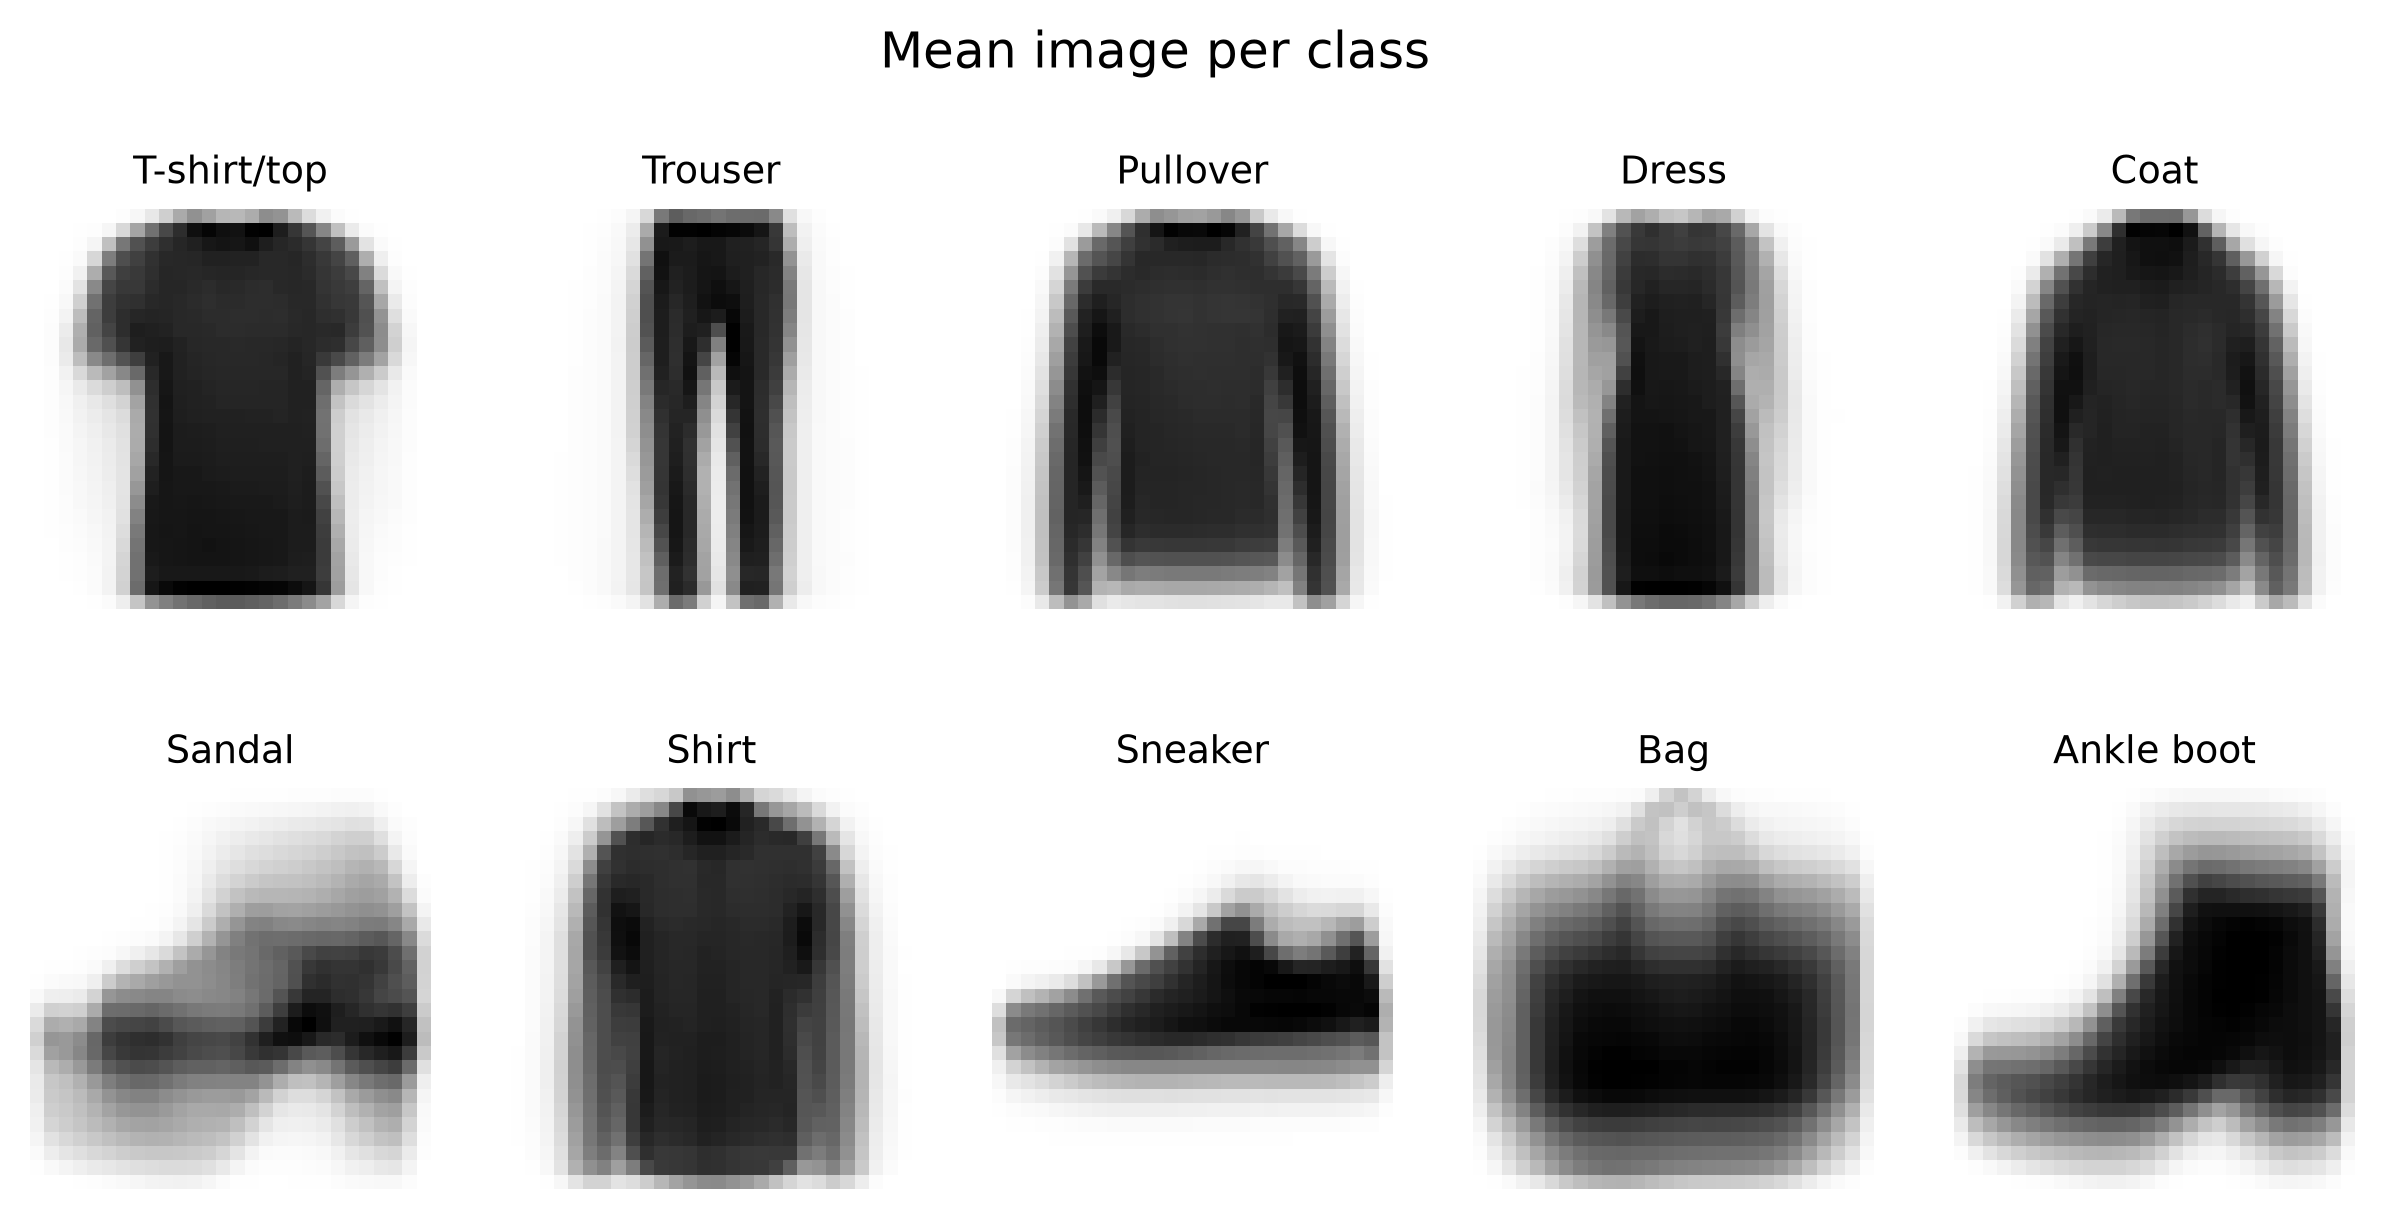
\includegraphics[width=\linewidth]{eda_class_mean_images.png}\\[2pt]
  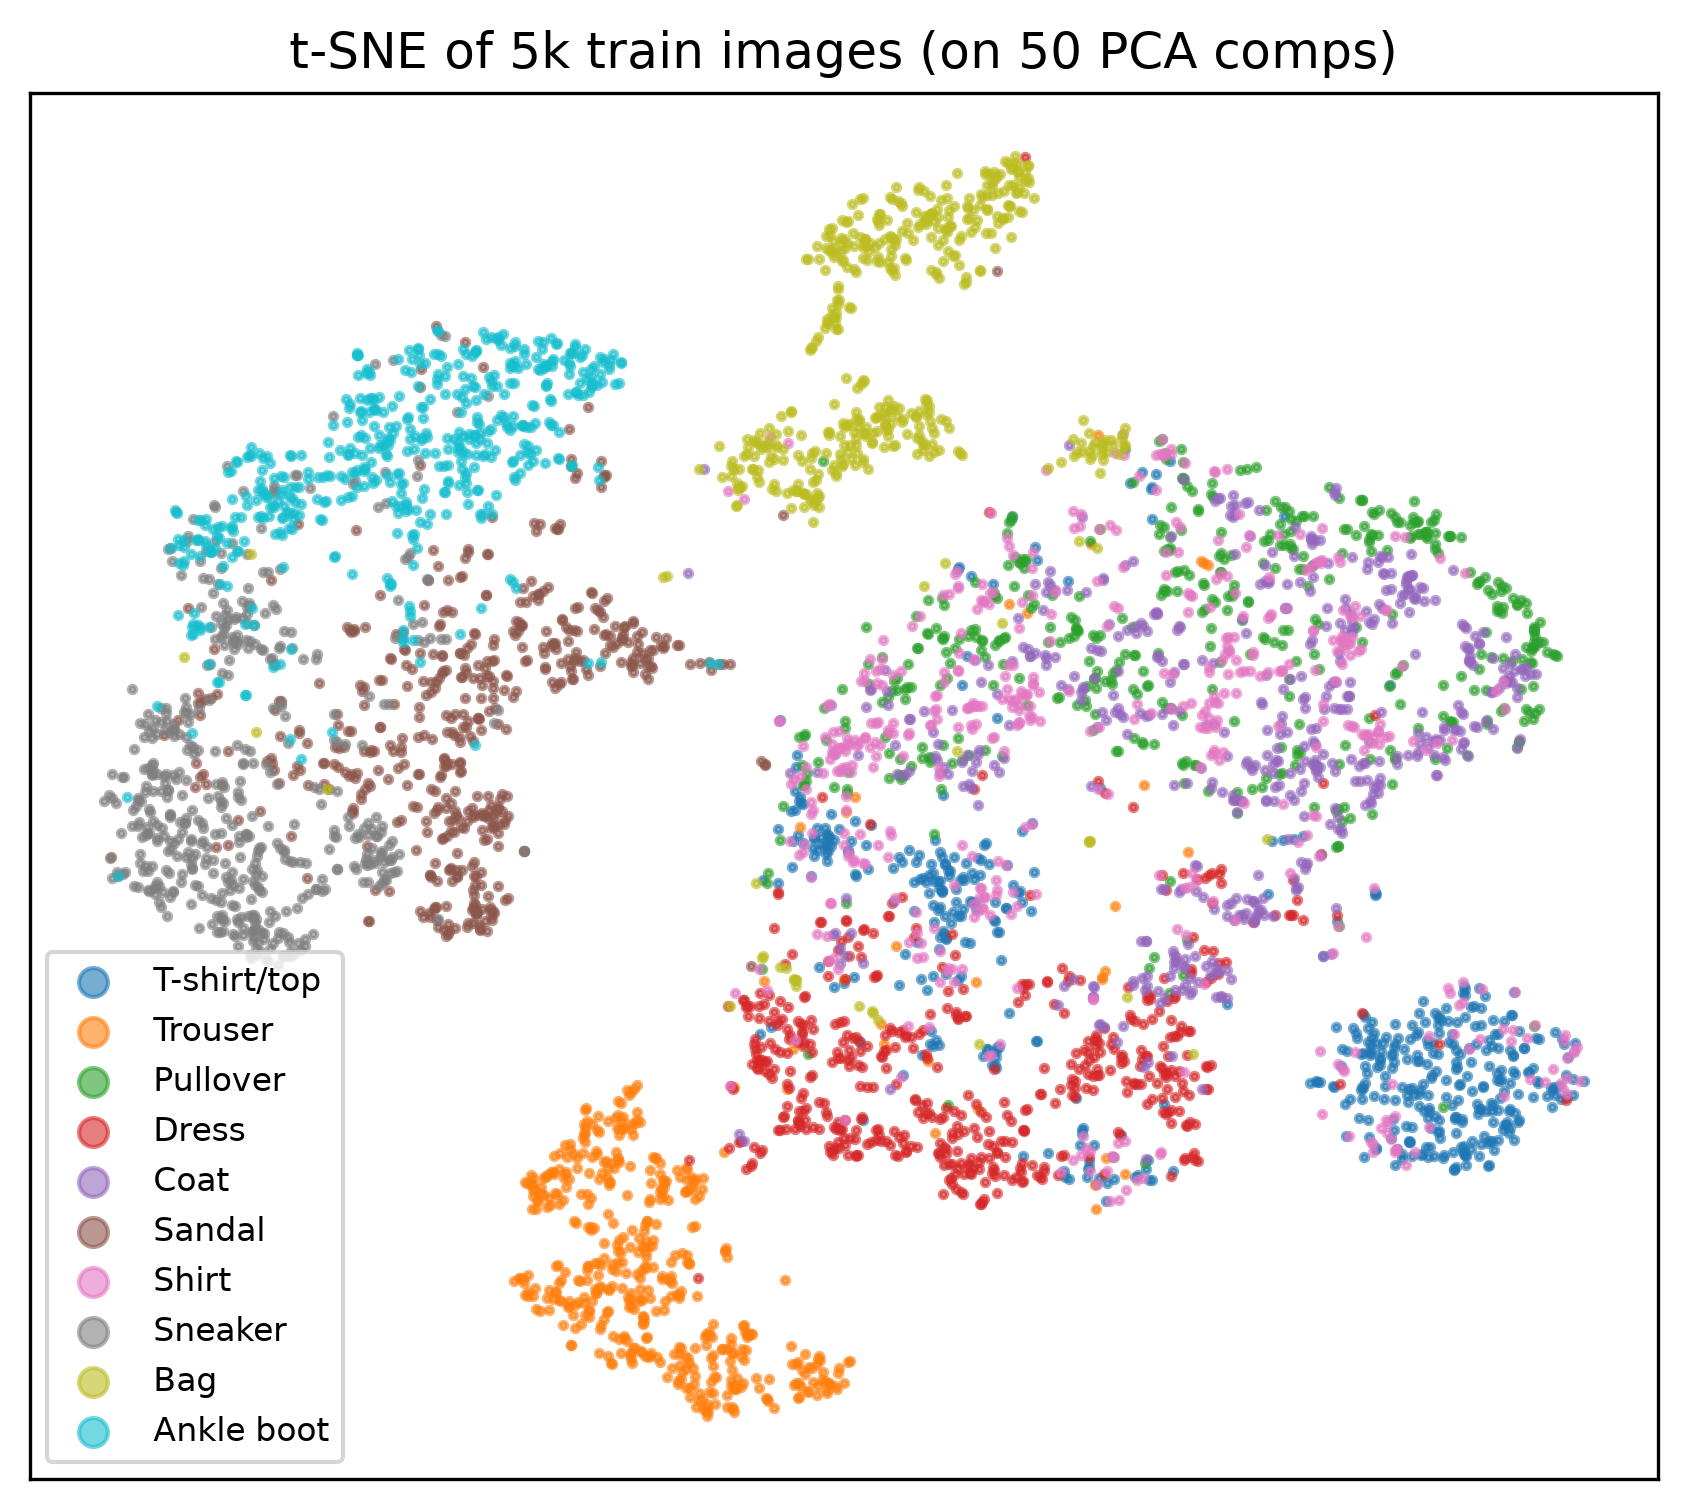
\includegraphics[width=0.85\linewidth]{eda_tsne.png}
  \caption{Top: mean image of each class (training split). Bottom: t-SNE map of a training subsample. Pullover, Coat and
  Shirt overlap; Trouser and Bag are well separated.}
  \label{fig:eda}
\end{figure}

% -------------------------------------------------------------------------------------
\section{Features}
\textbf{Pixels.} Each image is flattened to a 784-dimensional vector with values in $[0,1]$. Flattening discards the 2-D
neighbourhood: a garment shifted by two pixels becomes a very different vector.

\textbf{HOG settings sweep.} We tried $3\times2\times2=12$ HOG configurations: orientations $\{6,9,12\}$, cell size
$\{4\times4, 7\times7\}$ pixels and block size $\{1\times1, 2\times2\}$ cells. Each was scored by a fast proxy (a linear SVM
trained with SGD and hinge loss) fitted on training features and scored on validation (Table~\ref{tab:hog}). Small cells
win by 4--8 points, block normalisation adds 2--3 points and more orientation bins help slightly. The rule fixed in advance
was ``highest validation accuracy; within 0.3 points prefer the smaller vector''. The winner (12 orientations, $4\times4$
cells, $2\times2$ blocks, 1,728 dimensions, 0.8818) beats the 1,296-dimensional runner-up (0.8783) by 0.35 points, so it
was chosen. Extraction costs about 0.22\,s per 1,000 images.

\begin{table}[t]
  \centering
  \caption{HOG sweep: proxy validation accuracy (selected setting in bold; 7 of 12 configurations shown)}
  \label{tab:hog}
  \begin{tabular}{ccc r r}
    \toprule
    Orient. & Cell & Block & Dim. & Val acc \\
    \midrule
    6  & 4 & 2 & 864  & 0.8757 \\
    9  & 4 & 2 & 1296 & 0.8783 \\
    \textbf{12} & \textbf{4} & \textbf{2} & \textbf{1728} & \textbf{0.8818} \\
    12 & 4 & 1 & 588  & 0.8630 \\
    12 & 7 & 2 & 432  & 0.8357 \\
    12 & 7 & 1 & 192  & 0.8010 \\
    6  & 7 & 1 & 96   & 0.7612 \\
    \bottomrule
  \end{tabular}
\end{table}

\begin{figure}[t]
  \centering
  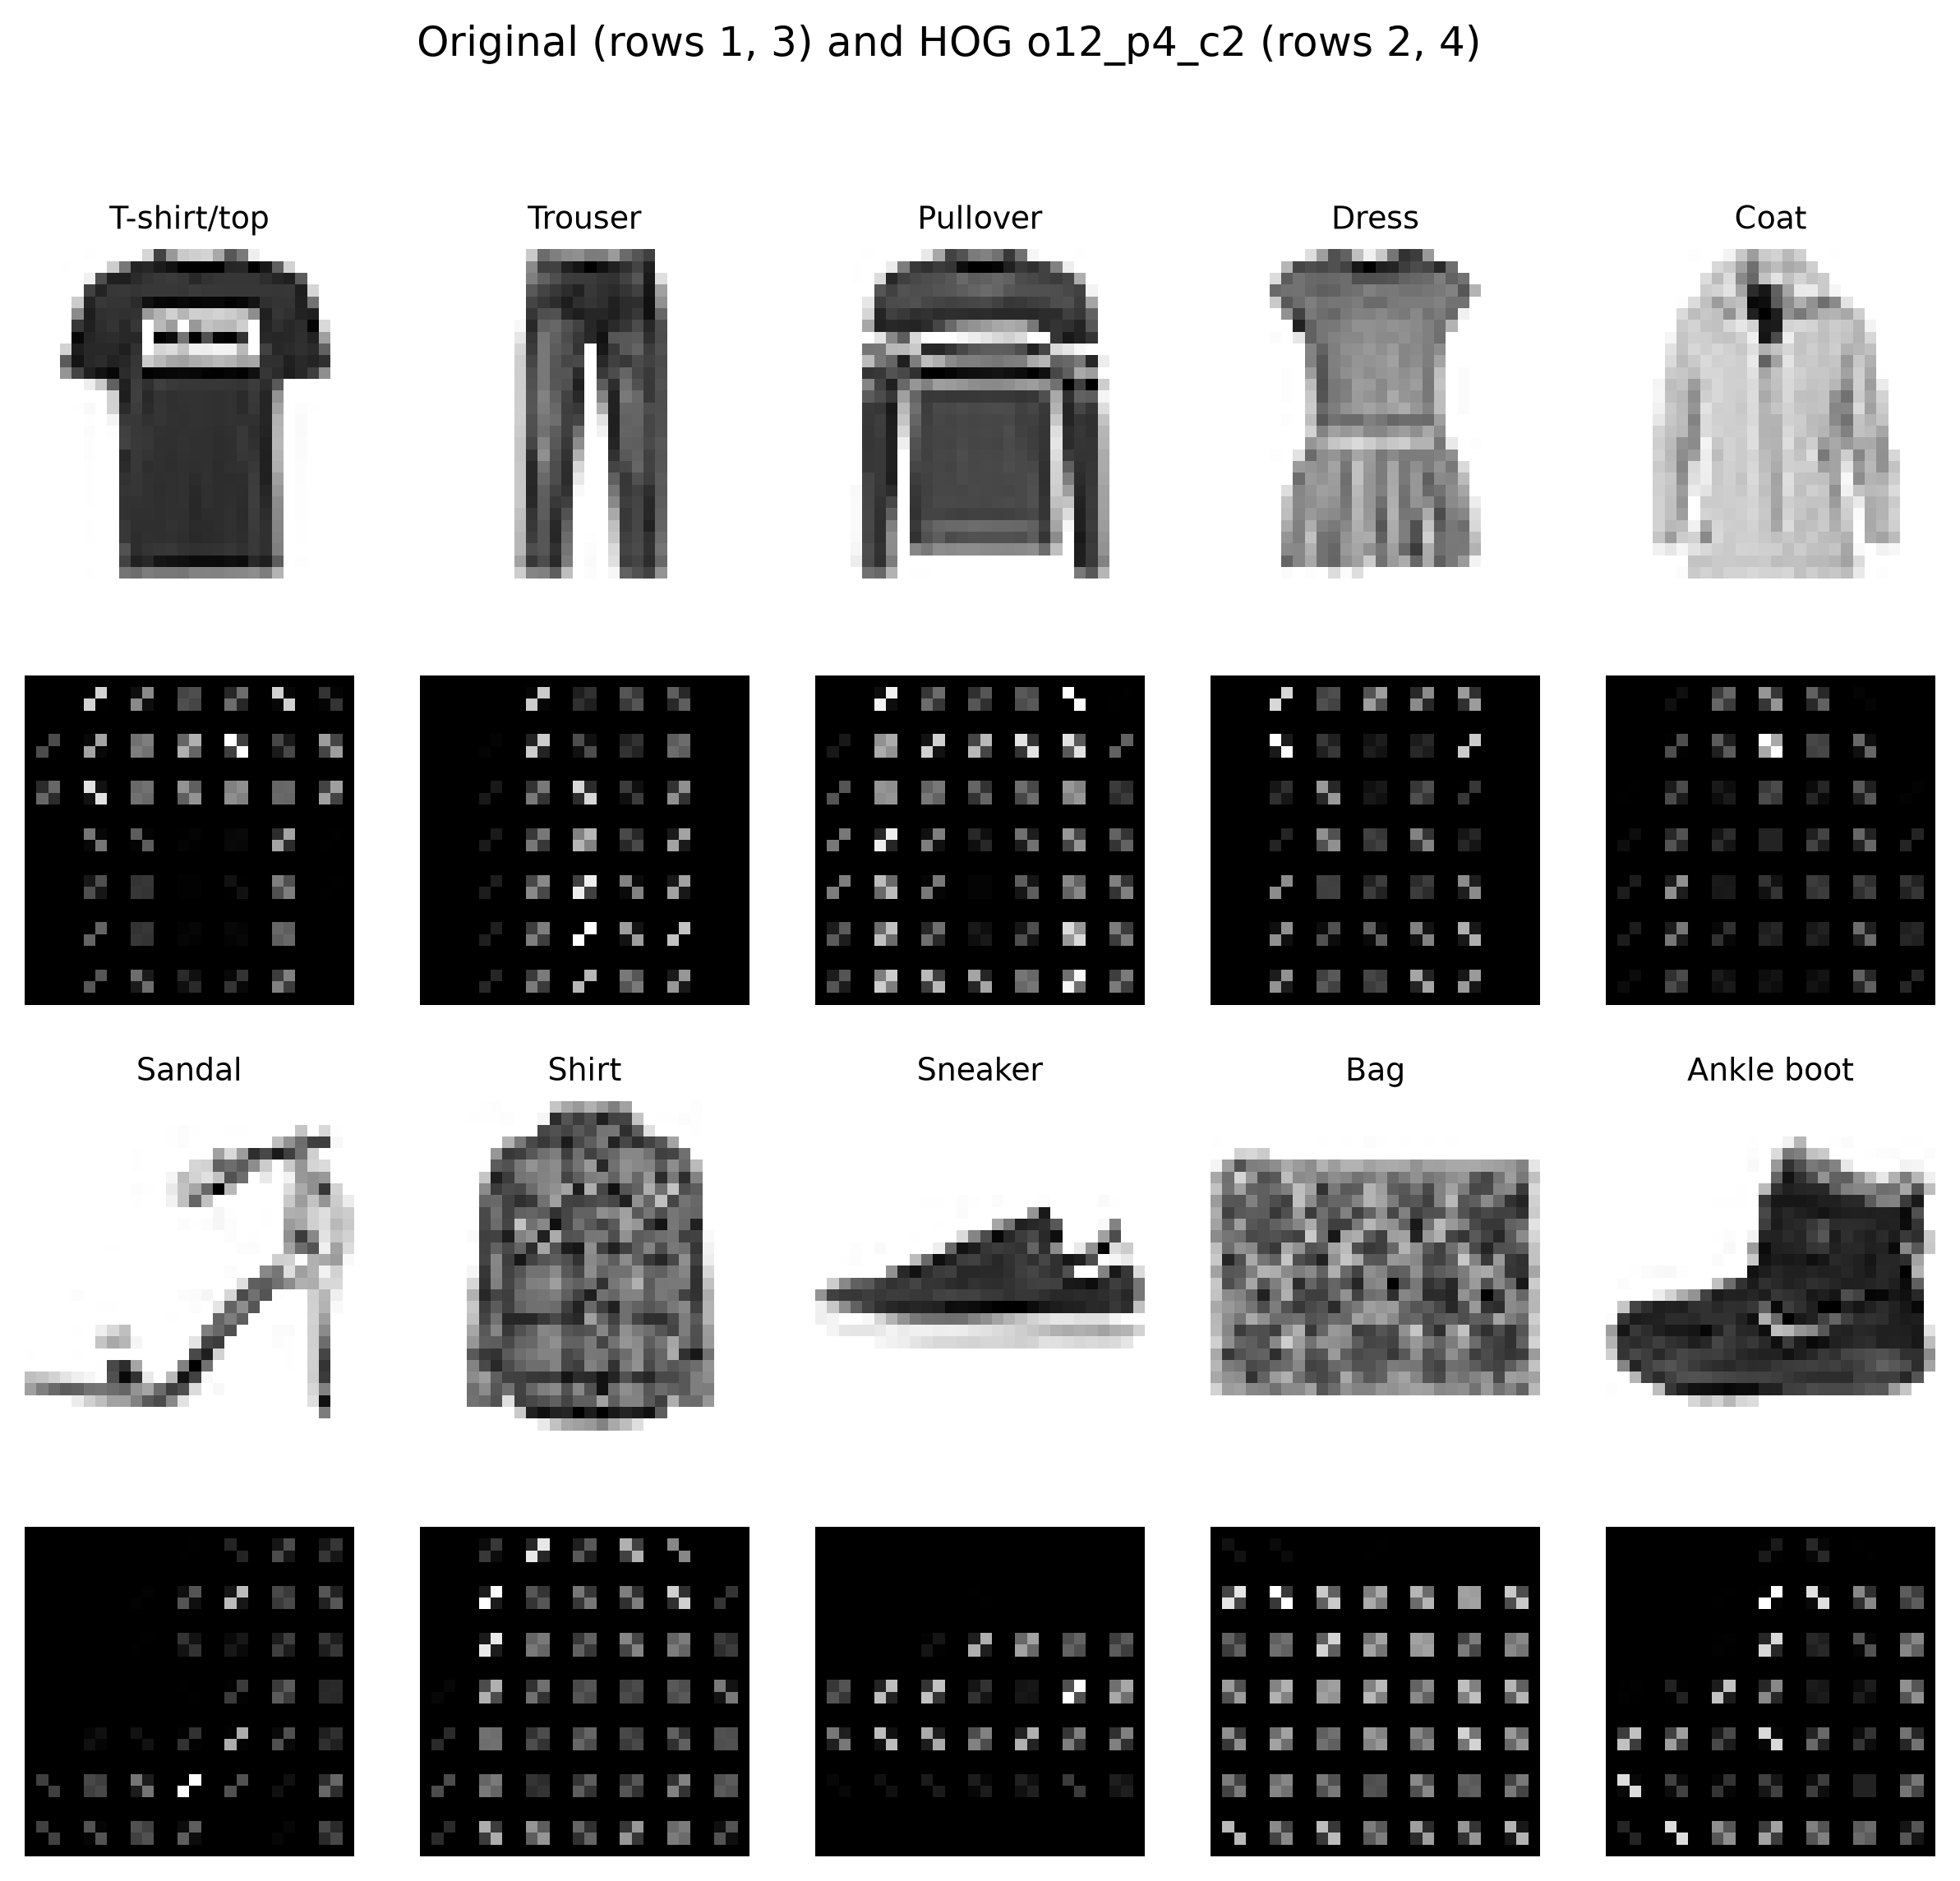
\includegraphics[width=\linewidth]{features_hog_examples.png}
  \caption{One training image per class next to its HOG descriptor. The four tops produce similar torso-and-sleeve edge
  patterns; shoes and trousers have distinctive edge layouts.}
  \label{fig:hog}
\end{figure}

\textbf{Scaling.} Logistic Regression, SVMs and $k$-NN are sensitive to feature scale, so they standardise features
inside their pipeline. Random Forest splits one feature at a time on a threshold, which rescaling does not change, so it
uses no scaler.

% -------------------------------------------------------------------------------------
\section{Models and Tuning}
Table~\ref{tab:grids} lists the validation grids and the selected settings. Two practical constraints shaped tuning on an
8\,GB laptop. First, the RBF SVM's training time grows faster than linearly with data, so its 9-combination grid was
searched on a stratified 10,000-image subset (1,000 per class), and only the selected setting was refit on all 60,000
images. Second, Linear SVM fits on 54,000 images took 105--924\,s, growing sharply with $C$.

\begin{table}[t]
  \centering
  \caption{Validation grids and selected settings}
  \label{tab:grids}
  \setlength{\tabcolsep}{3pt}
  \begin{tabular}{p{1.45cm} p{3.05cm} p{2.9cm}}
    \toprule
    Model & Grid & Selected (pixels / HOG) \\
    \midrule
    Log.\ Reg. & $C\in\{0.01,0.1,1,10\}$ & $C=0.01$ / $C=0.01$ \\
    $k$-NN & $k\in\{1,3,5,7,9\}$, uniform/distance, Euclid./Manhattan & $k=3$, distance, Manhattan / $k=3$, distance, Euclidean \\
    Rand.\ Forest & trees $\{100,300\}$, depth $\{\text{None},20,40\}$, features $\{\sqrt{p},\log_2 p\}$ & 300, depth 20, $\sqrt{p}$ / 300, full depth, $\sqrt{p}$ \\
    Linear SVM & $C\in\{0.01,0.1,1\}$ & $C=0.01$ / $C=0.01$ \\
    RBF SVM & $C\in\{0.1,1,10\}$, $\gamma\in\{\text{scale},0.01,0.001\}$ (10k subset) & $C=10,\gamma=0.001$ / $C=10,\gamma=\text{scale}$ \\
    \bottomrule
  \end{tabular}
\end{table}

\textbf{A fair validation comparison.} Because the RBF SVM was tuned on 10,000 images, its tuning validation scores
(0.8793 pixels, 0.8867 HOG) came from less training data than every other model's (54,000) and understated it. Before
choosing the best model, we wrote down the fix: refit the \emph{already selected} RBF settings on the full 54,000-image
training split and score them on the same validation set, with no new search and no test data. This gave 0.9082 (pixels)
and 0.9157 (HOG). With all scores on an equal footing, the validation ranking is RBF SVM HOG (0.9157) $>$ RBF SVM pixels
(0.9082) $>$ Logistic Regression HOG (0.8927) $>$ Linear SVM HOG (0.8900).

\textbf{Observations.} The best $C$ sits at the edge of the grid for Logistic Regression and Linear SVM (0.01, the
smallest) and for the RBF SVM (10, the largest). We did not widen the grids afterwards, to avoid another round of test
evaluation; this is a limitation. For the RBF SVM, $\gamma=0.01$ is far too narrow for standardised 784- or
1,728-dimensional inputs: HOG validation accuracy collapses to 11--29\%.

% -------------------------------------------------------------------------------------
\section{Results}
Table~\ref{tab:results} lists all 12 experiments. Pixel results are in line with the baselines reported with the
dataset~\cite{xiao2017fashion}.

\begin{table*}[t]
  \centering
  \caption{All experiments. Val acc: model trained on 54k (RBF SVM refit on 54k for comparability). Test metrics: final
  model trained on 60k, evaluated once. Inference is model-only time per 1,000 test images; HOG extraction adds about 216\,ms.}
  \label{tab:results}
  \begin{tabular}{l l c c c r r r}
    \toprule
    Model & Features & Val acc & Test acc & Macro F1 & Train (s) & Inference (ms/1k) & Size \\
    \midrule
    Dummy (most frequent) & Pixels & 0.1000 & 0.1000 & 0.0182 & 0.00 & 0.00$^{a}$ & 709\,B \\
    Dummy (most frequent) & HOG    & 0.1000 & 0.1000 & 0.0182 & 0.16 & 0.01$^{a}$ & 709\,B \\
    Logistic Regression & Pixels & 0.8642 & 0.8472 & 0.8464 & n/a$^{b}$ & n/a$^{b}$ & 51.4\,KB \\
    Logistic Regression & HOG    & 0.8927 & 0.8886 & 0.8885 & n/a$^{b}$ & n/a$^{b}$ & 111.8\,KB \\
    $k$-NN & Pixels & 0.8747 & 0.8611 & 0.8614 & 0.49 & 6,926.61 & 188.7\,MB \\
    $k$-NN & HOG    & 0.8728 & 0.8631 & 0.8623 & 1.29 & 731.13 & 415.2\,MB \\
    Random Forest & Pixels & 0.8867 & 0.8756 & 0.8741 & 32.83 & 12.16 & 366.5\,MB \\
    Random Forest & HOG    & 0.8735 & 0.8703 & 0.8692 & 68.53 & 19.02 & 500.7\,MB \\
    Linear SVM & Pixels & 0.8583 & 0.8378 & 0.8353 & 99.24 & 1.22 & 82.7\,KB \\
    Linear SVM & HOG    & 0.8900 & 0.8898 & 0.8892 & 162.04 & 2.62 & 180.8\,KB \\
    RBF SVM & Pixels & 0.9082 & 0.8970 & 0.8967 & 195.67 & 4,766.94 & 125.1\,MB \\
    \textbf{RBF SVM} & \textbf{HOG} & \textbf{0.9157} & \textbf{0.9108} & \textbf{0.9108} & 451.43 & 28,876.96$^{c}$ & 366.2\,MB \\
    \bottomrule
    \multicolumn{8}{l}{\footnotesize $^{a}$Measured on a different machine; excluded from speed comparisons.
    $^{b}$Not comparable (runs overlapped other work); accuracy unaffected.}\\
    \multicolumn{8}{l}{\footnotesize $^{c}$26,343 support vectors; looks about $2\times$ slower than expected, so treated as an upper bound.
    $k$-NN timed on an Apple M3; Random Forest and SVMs on an Apple M3 Pro.}
  \end{tabular}
\end{table*}

\subsection{RQ1: Raw pixels}
The best pixel model is the RBF SVM at 89.70\%. Random Forest reaches 87.56\%, $k$-NN 86.11\%, and the linear models
only 83.78--84.72\%. A single pixel only records the brightness of one location, so a linear boundary in pixel space cannot
capture shape.

\subsection{RQ2: HOG vs.\ pixels}
HOG helps the linear models most: +5.20 points for Linear SVM (83.78\%\,$\rightarrow$\,88.98\%) and +4.14 for Logistic
Regression (84.72\%\,$\rightarrow$\,88.86\%). It lifts the RBF SVM by +1.38 to 91.08\%. It does not help Random Forest
($-0.53$) or $k$-NN ($+0.20$) (Fig.~\ref{fig:rq23}, left). A plausible explanation for the forest is that each split looks
at one feature, and one raw pixel is more informative on its own than one HOG bin, which describes one edge direction in
one small block. We did not test this explanation directly.

\begin{figure*}[t]
  \centering
  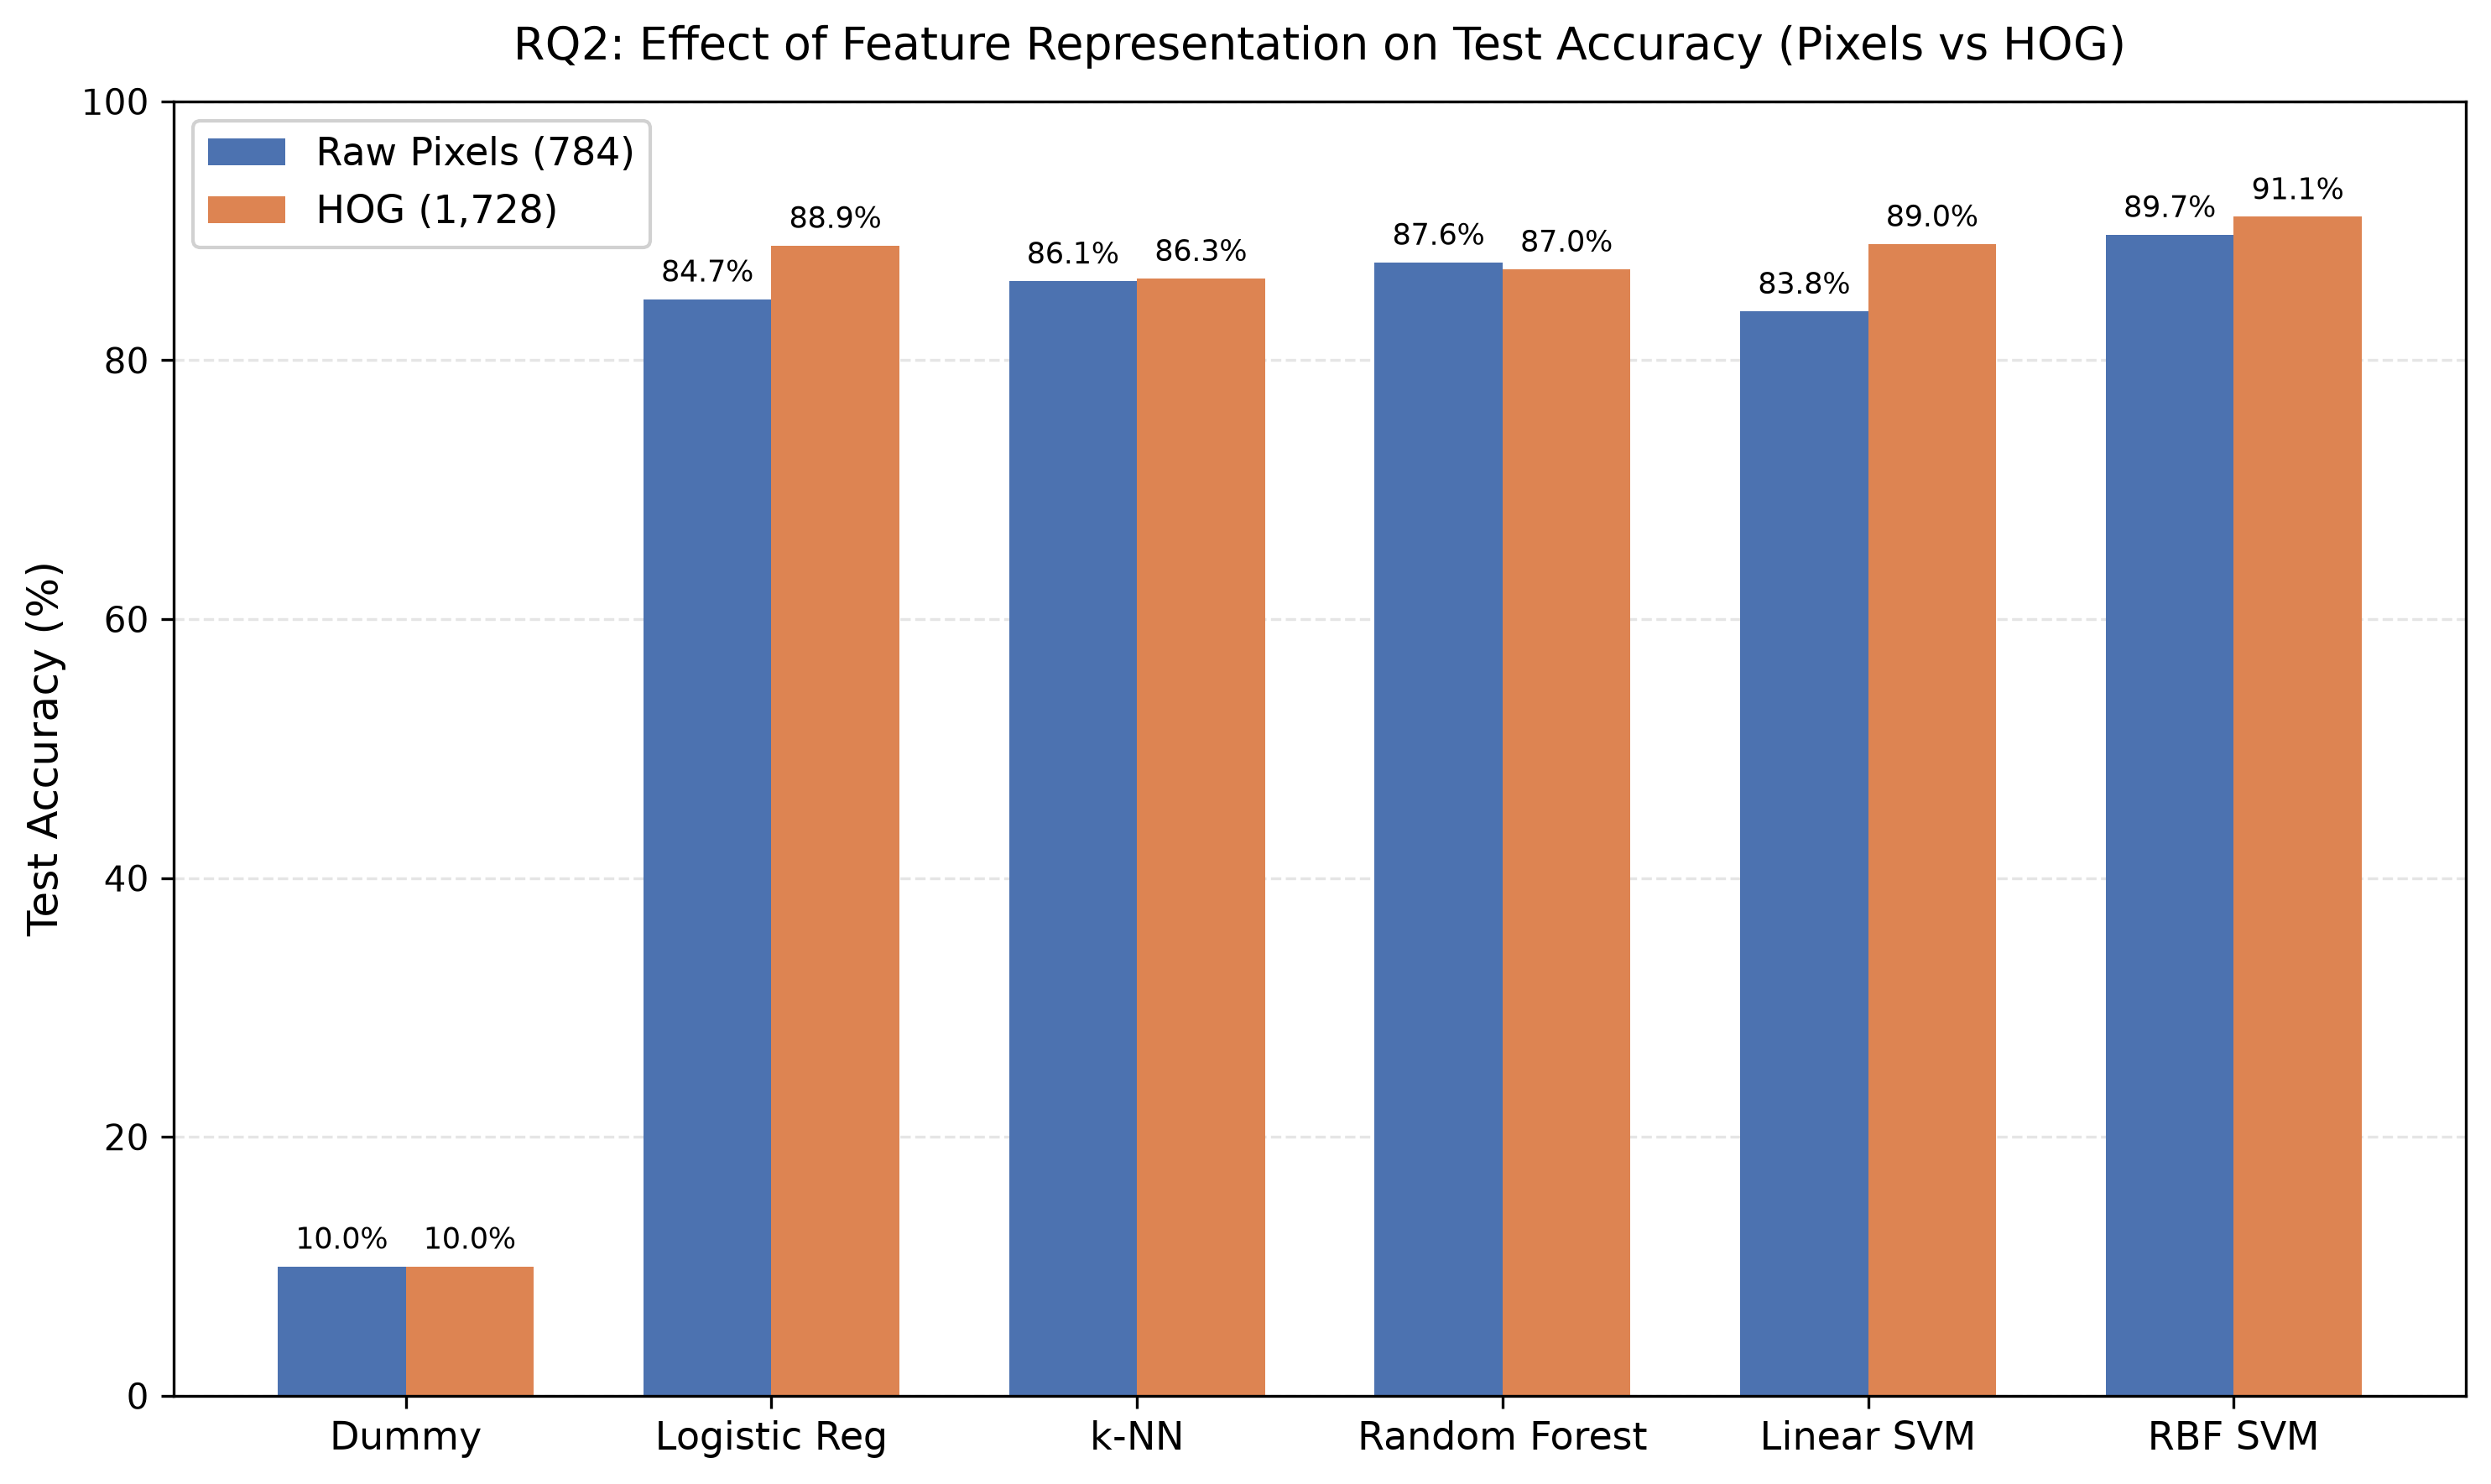
\includegraphics[width=0.48\linewidth]{results_pixels_vs_hog.png}\hfill
  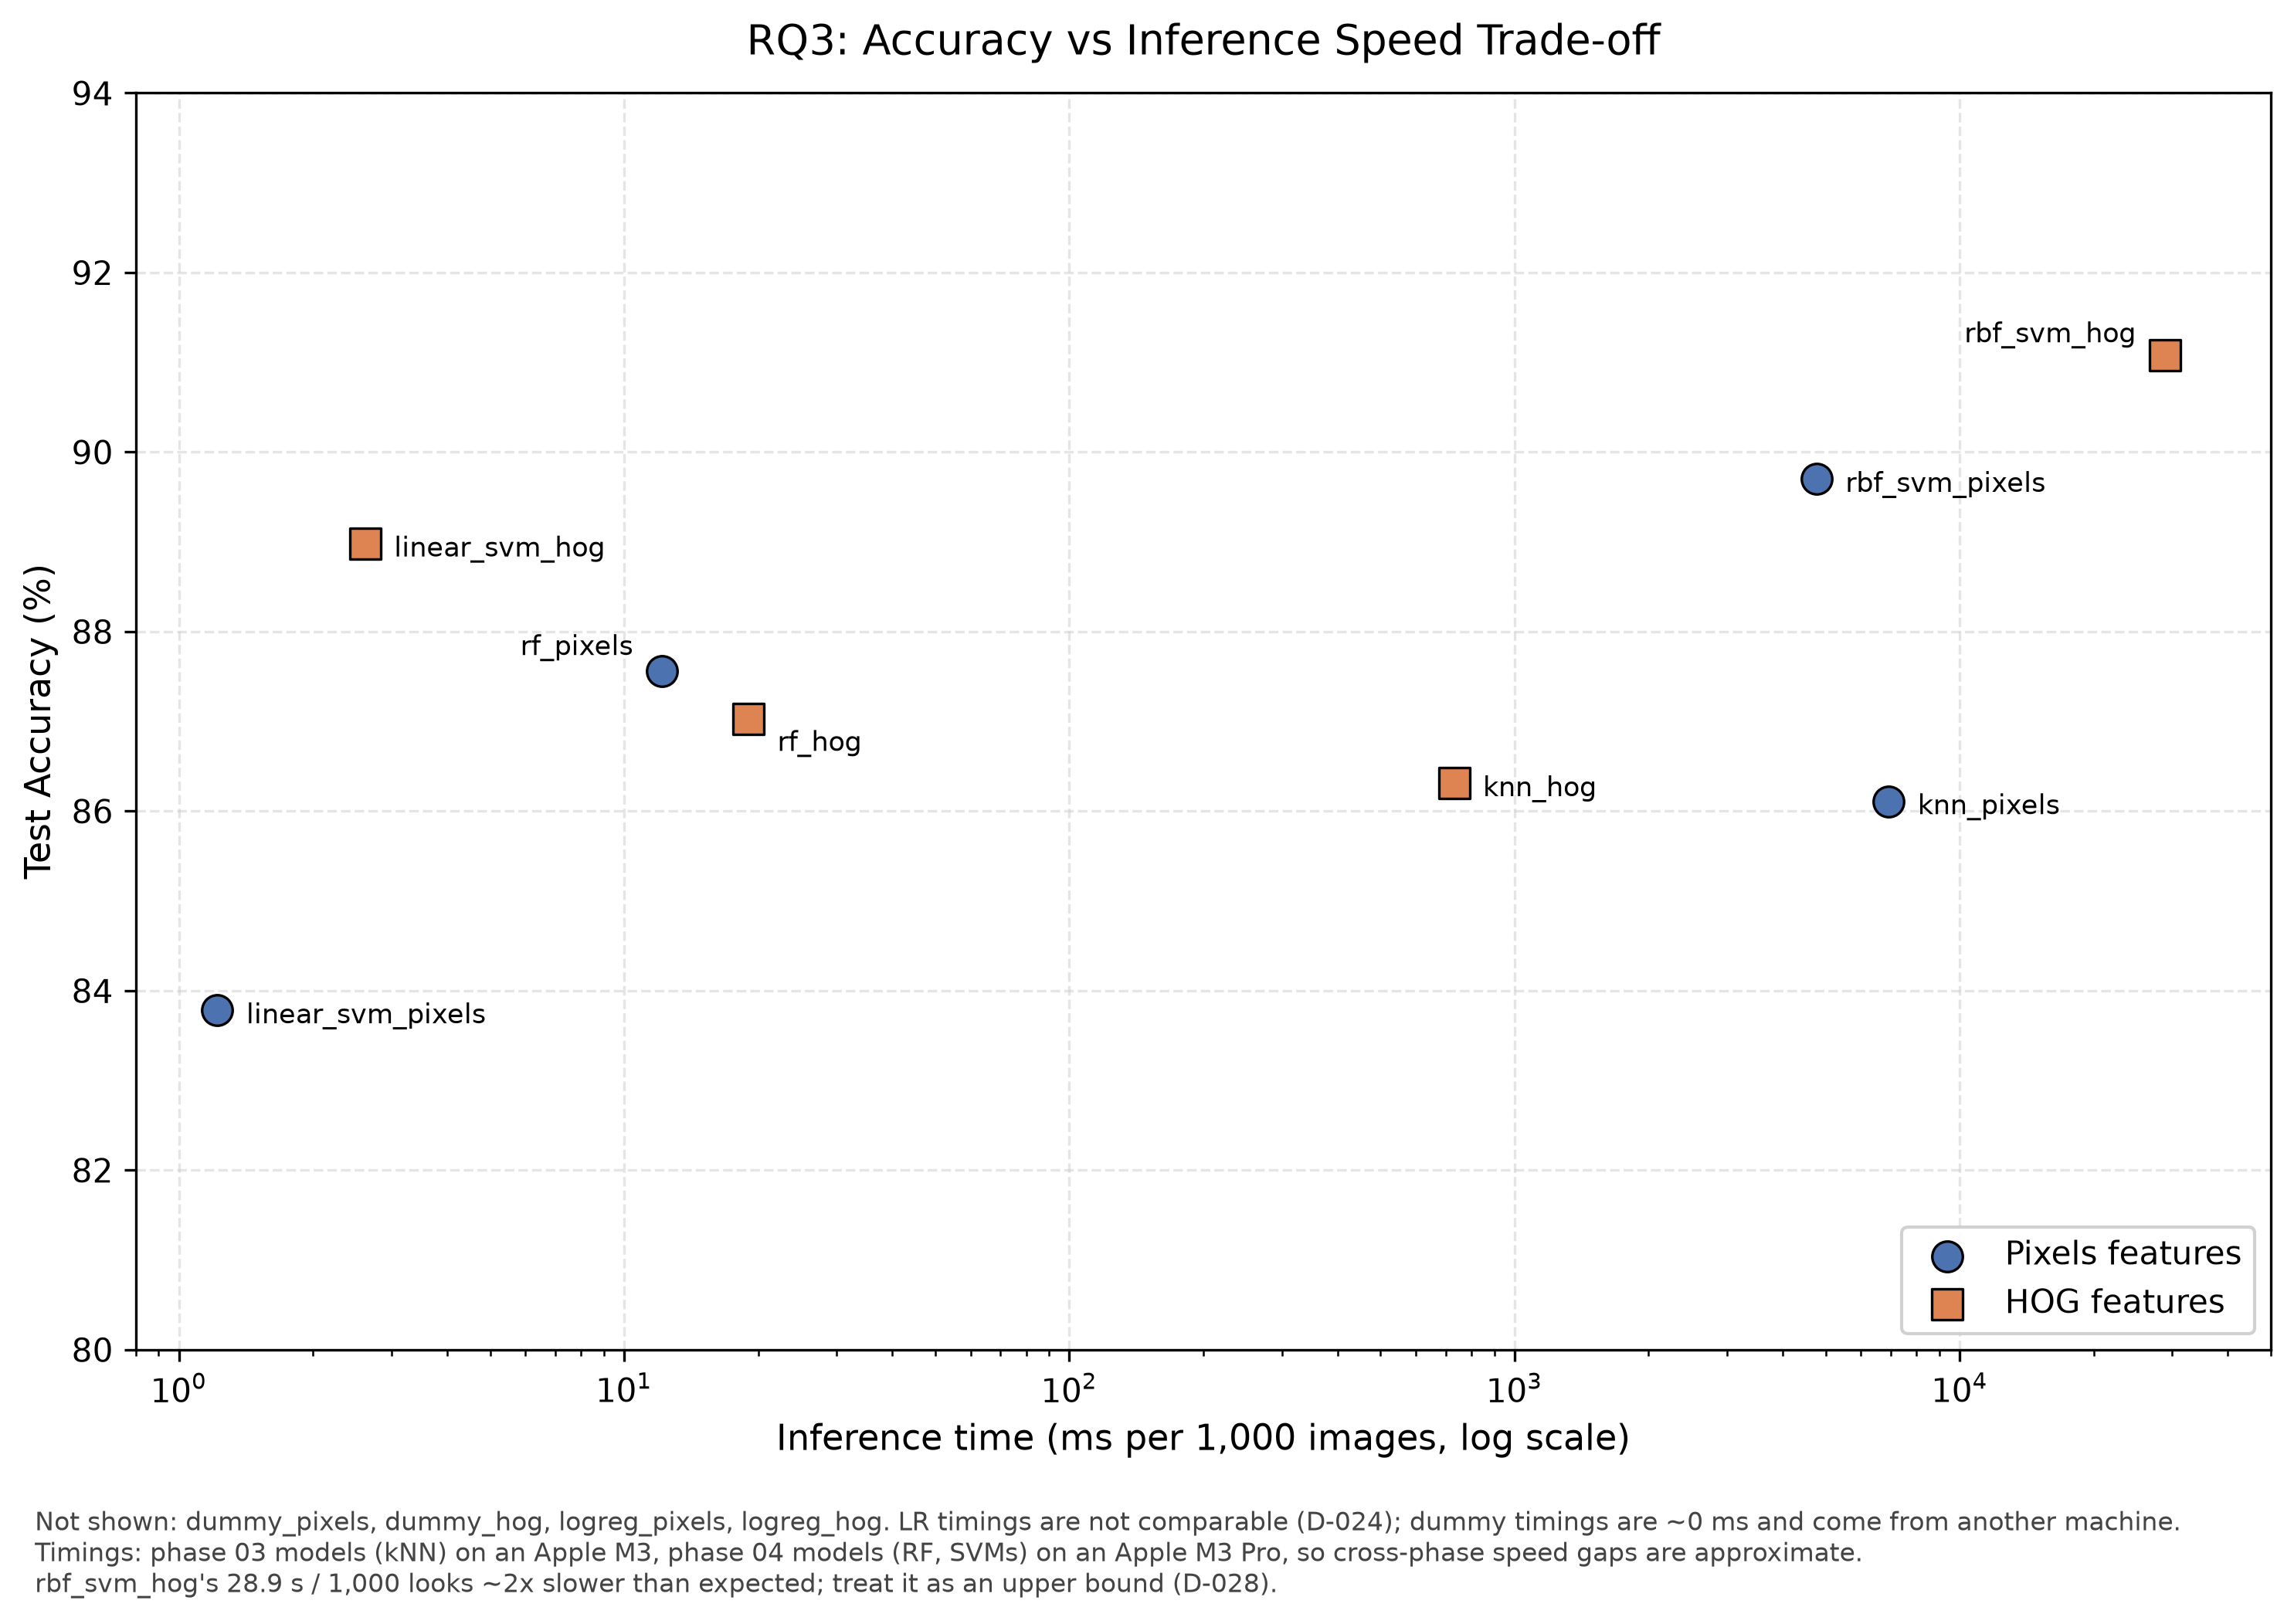
\includegraphics[width=0.48\linewidth]{results_acc_vs_time.png}
  \caption{Left: test accuracy with pixels vs.\ HOG features (RQ2). Right: test accuracy vs.\ model-only prediction time
  per 1,000 images, log scale (RQ3). Logistic Regression and the dummy baseline are excluded from the speed plot.}
  \label{fig:rq23}
\end{figure*}

\subsection{RQ3: Accuracy, speed and size}
A fair speed comparison must include feature extraction. Counting about 216\,ms per 1,000 images for HOG, the
end-to-end picture is:
\begin{itemize}
  \item \textbf{Fastest above 87\%:} Random Forest on pixels, 87.56\% in about 12\,ms per 1,000 images, but the model is
        366\,MB.
  \item \textbf{Best accuracy for its size:} Linear SVM on HOG, 88.98\% with a 181\,KB model; its 219\,ms per 1,000
        images is almost entirely HOG extraction.
  \item \textbf{Most accurate:} RBF SVM on HOG, 91.08\%, but about 29\,s per 1,000 images, about 2,400 times slower than the
        Random Forest for +3.5 points. Each prediction is compared with all 26,343 support vectors.
\end{itemize}
$k$-NN is both slower and less accurate than the Random Forest, so it is never the best choice here.

\subsection{Selected model and stability}
The best model by validation accuracy is the RBF SVM on HOG (validation 0.9157). The test score played no part in this
choice. Validation accuracy on 6,000 images has a standard error of about $\pm0.4$ points, so its 0.75-point lead over the
pixel RBF SVM is real but modest. A stratified 5-fold cross-validation on a 10,000-image subset of the training and
validation data gives $0.8775\pm0.0054$ (folds 0.8765, 0.8860, 0.8715, 0.8725, 0.8810). The low spread shows the model is
stable across data partitions; the lower mean is expected because each fold trains on only 8,000 images.

% -------------------------------------------------------------------------------------
\section{Error Analysis (RQ4)}
\textbf{Per-class recall.} Shirt is the hardest class for all ten trained models, with recall from 50.9\% (Linear SVM,
pixels) to 75.2\% (RBF SVM, HOG). Pullover (73.5--84.9\%) and Coat (76.4--86.3\%) follow. Trouser, Bag, Sandal, Sneaker
and Ankle boot are easy for every model (Fig.~\ref{fig:errors}, left).

\textbf{Top confusions of the best model.} From the saved confusion matrix (1,000 test images per class): Shirt\,$\rightarrow$\,T-shirt/top
(104), T-shirt/top\,$\rightarrow$\,Shirt (91), Pullover\,$\rightarrow$\,Shirt (66), Pullover\,$\rightarrow$\,Coat (61) and
Shirt\,$\rightarrow$\,Coat (59) (Fig.~\ref{fig:errors}, right). Mistakes among T-shirt/top, Pullover, Coat and Shirt
account for 56--66\% of every trained model's errors. This is exactly the group the EDA flagged before any model was
trained.

\begin{figure*}[t]
  \centering
  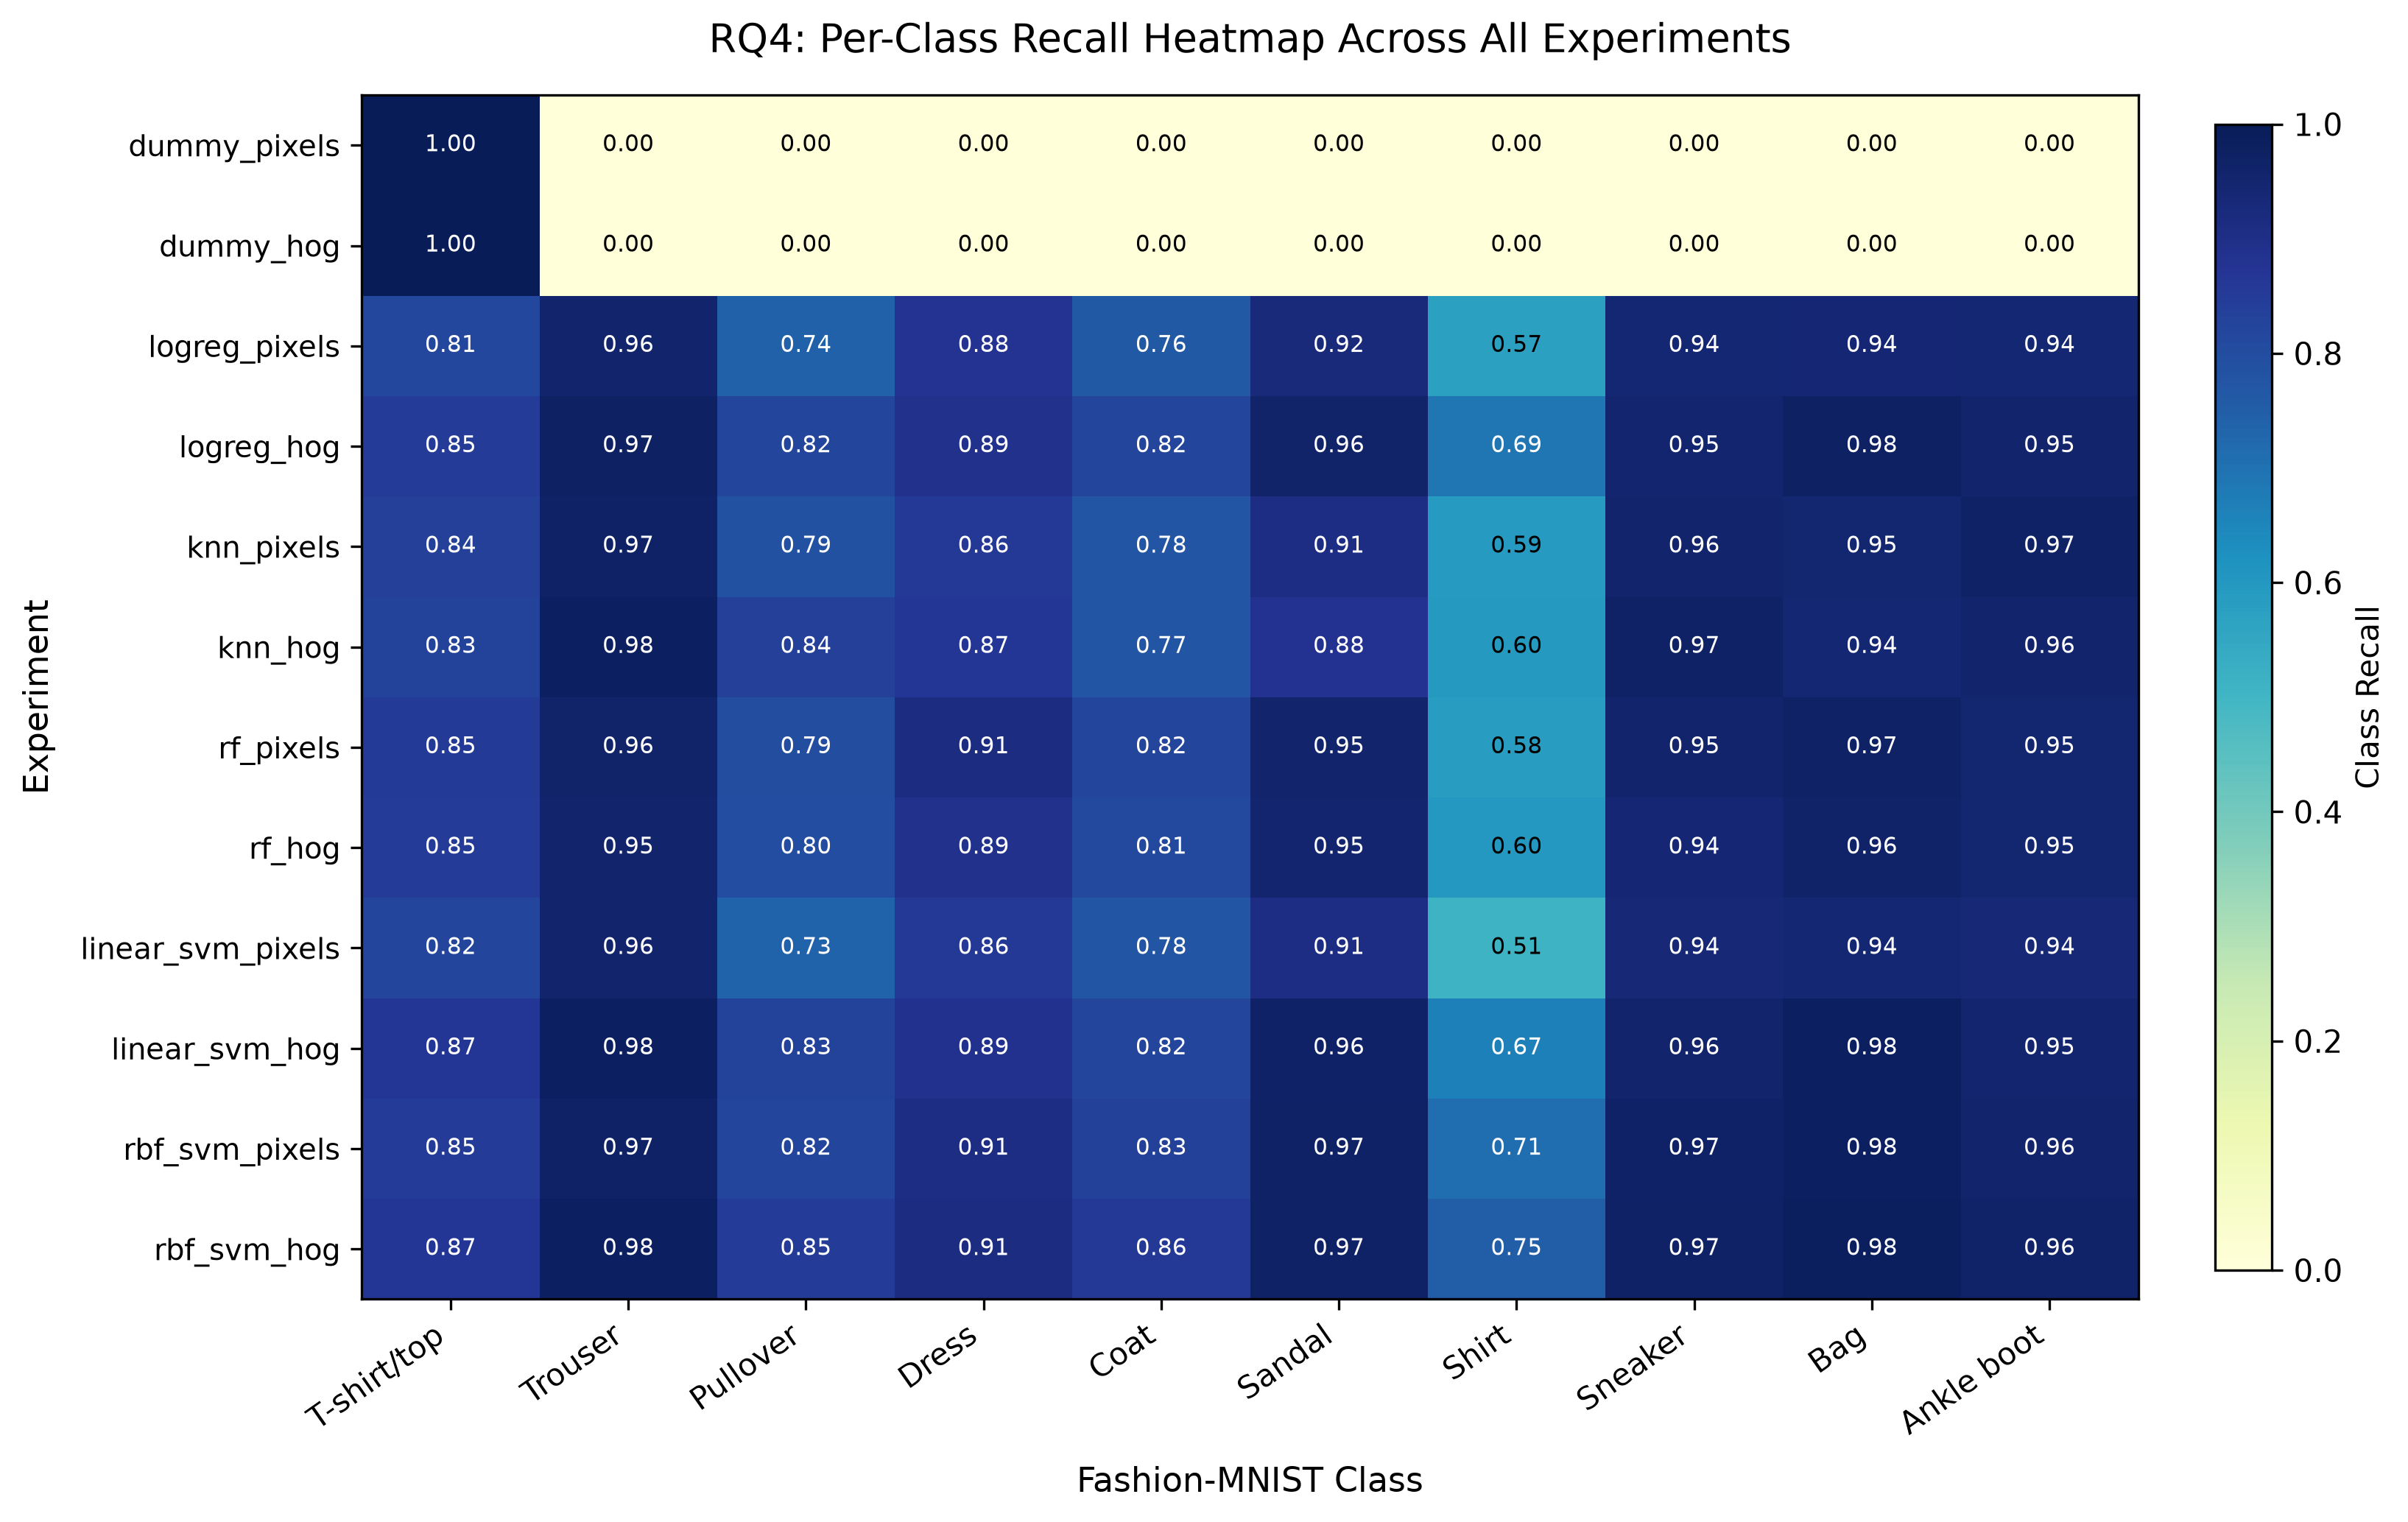
\includegraphics[width=0.52\linewidth]{results_recall_heatmap.png}\hfill
  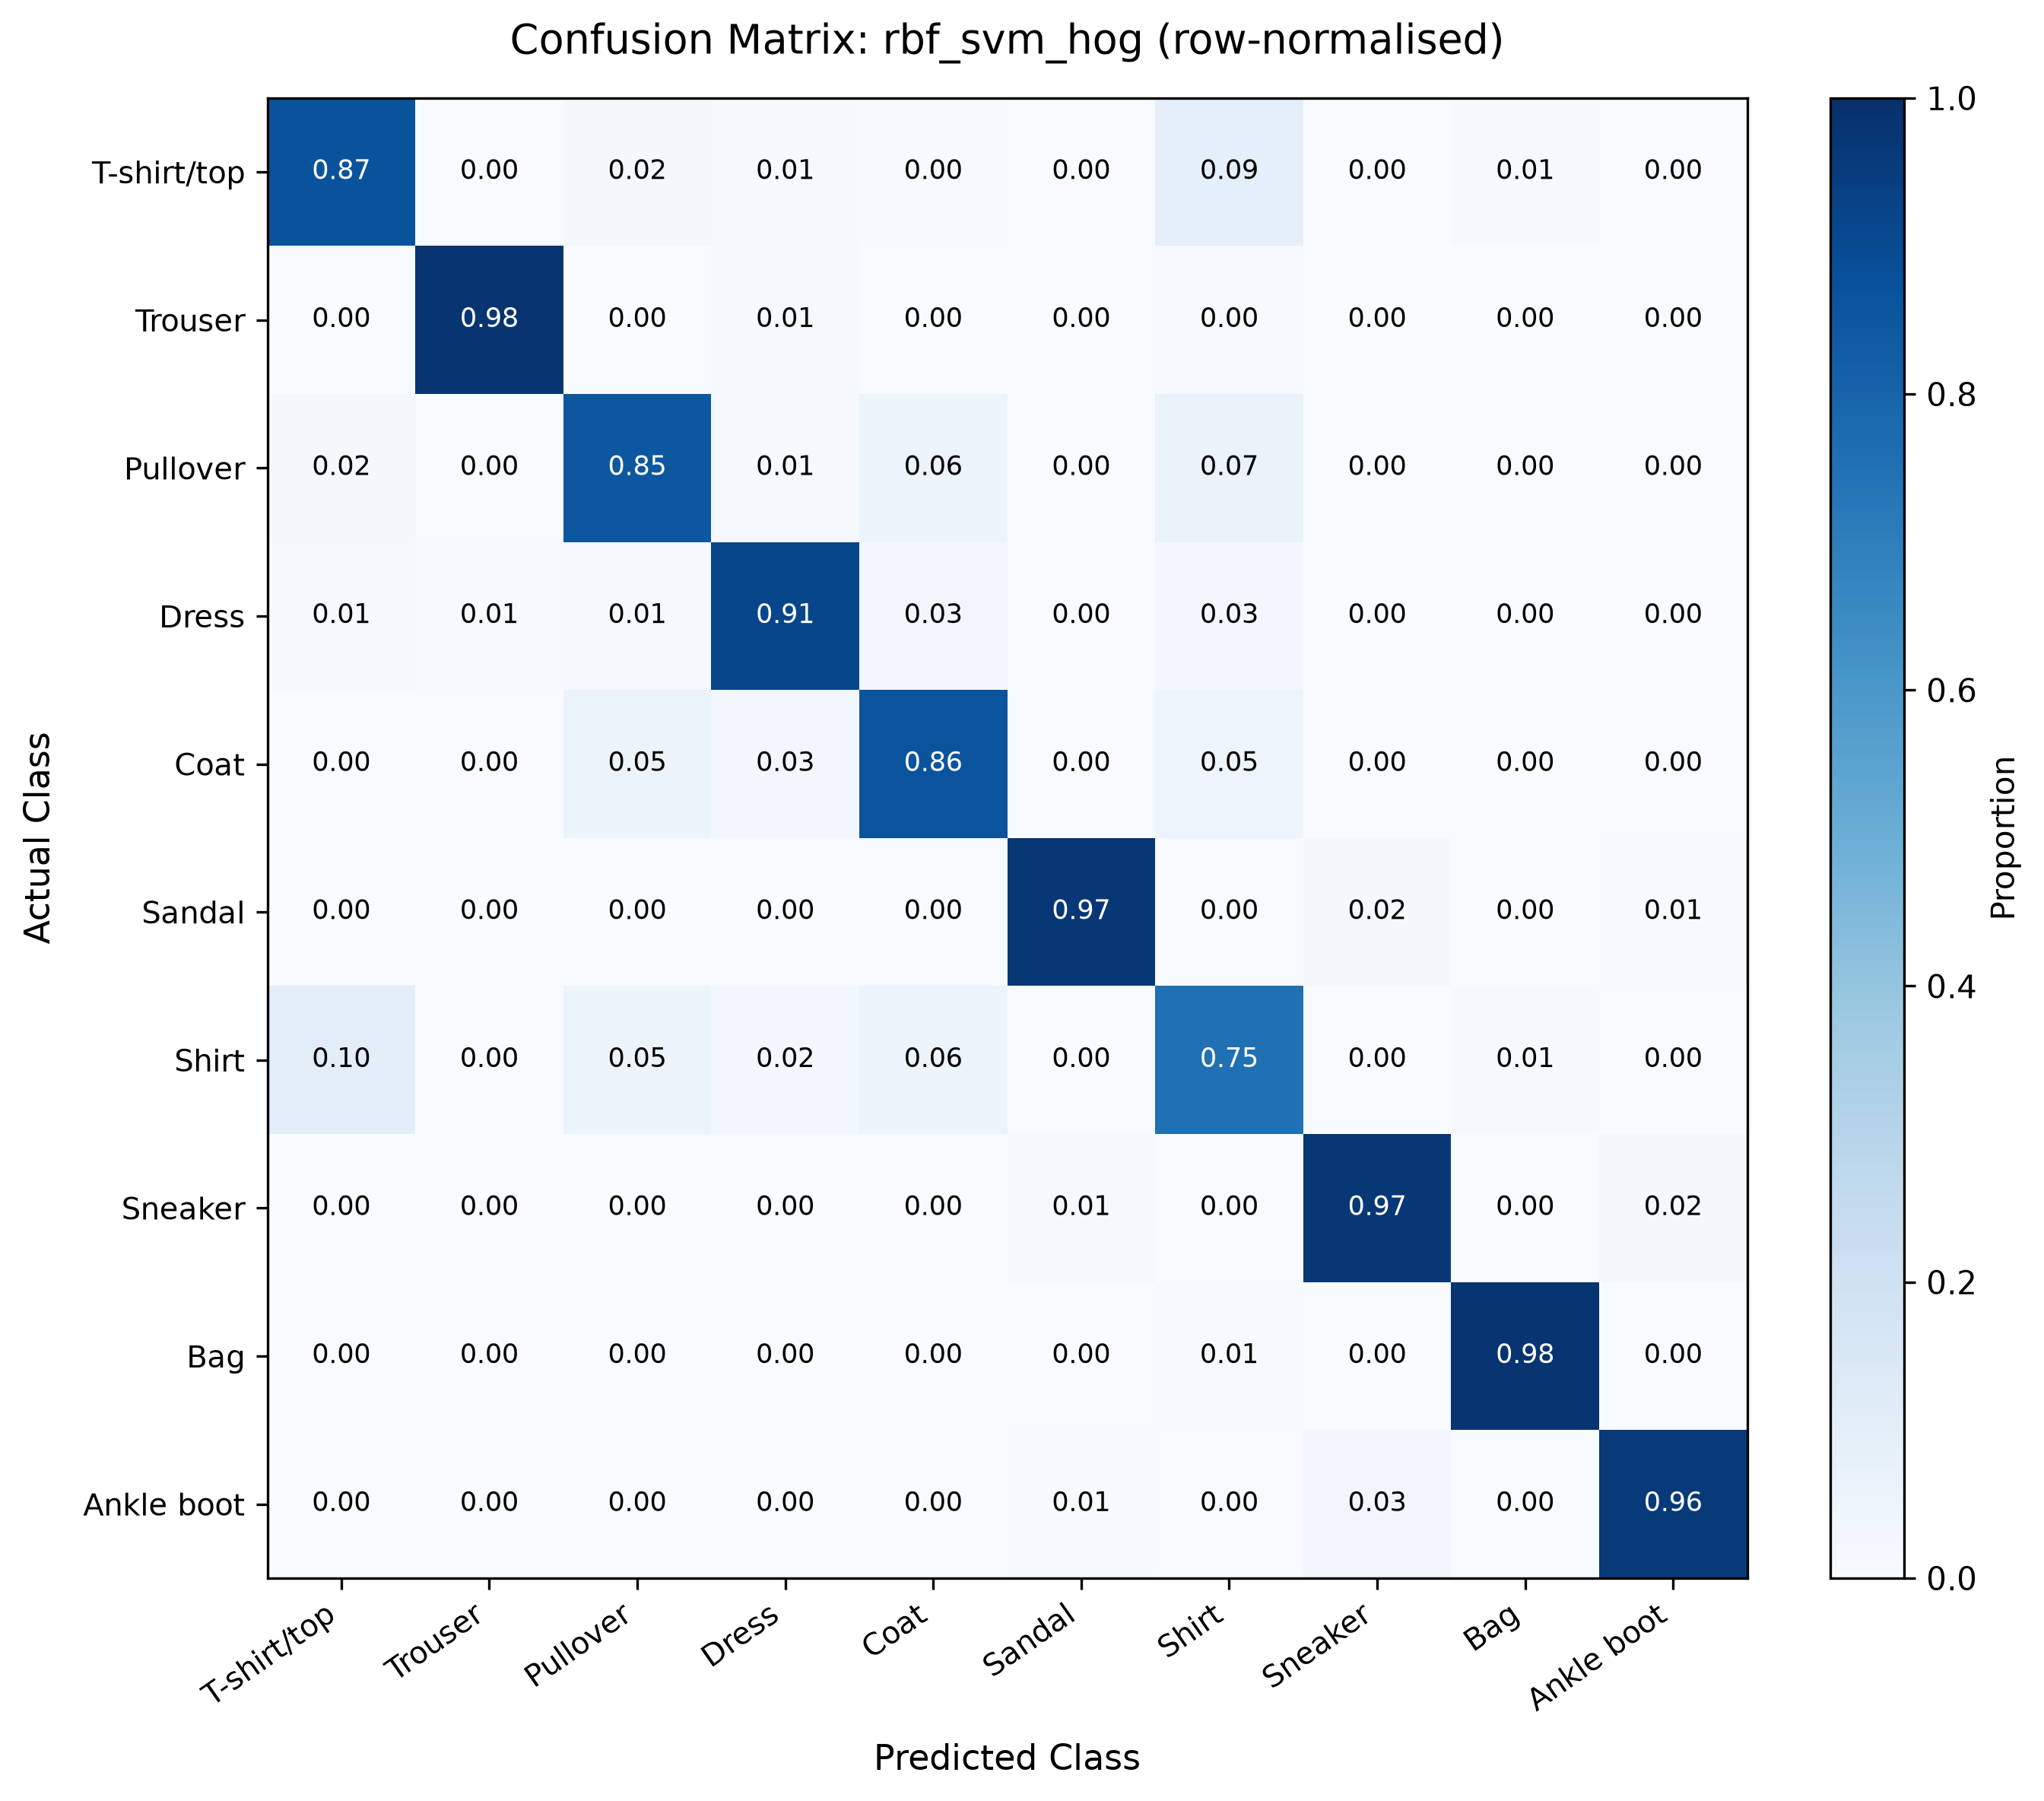
\includegraphics[width=0.44\linewidth]{errors_confusion_rbf_svm_hog.png}
  \caption{Left: per-class recall of all 12 experiments. Right: row-normalised confusion matrix of the selected model
  (RBF SVM, HOG). The upper-body garments form the main block of errors.}
  \label{fig:errors}
\end{figure*}

\textbf{Misclassified images.} Fig.~\ref{fig:mis} shows the first 16 test shirts (in test-set order, not hand-picked)
predicted as T-shirt/top. Many are short-sleeved, collarless or patterned; at $28\times28$ the collar and buttons that
define a shirt cover only a few pixels, and some images are ambiguous even to a person.

\begin{figure}[t]
  \centering
  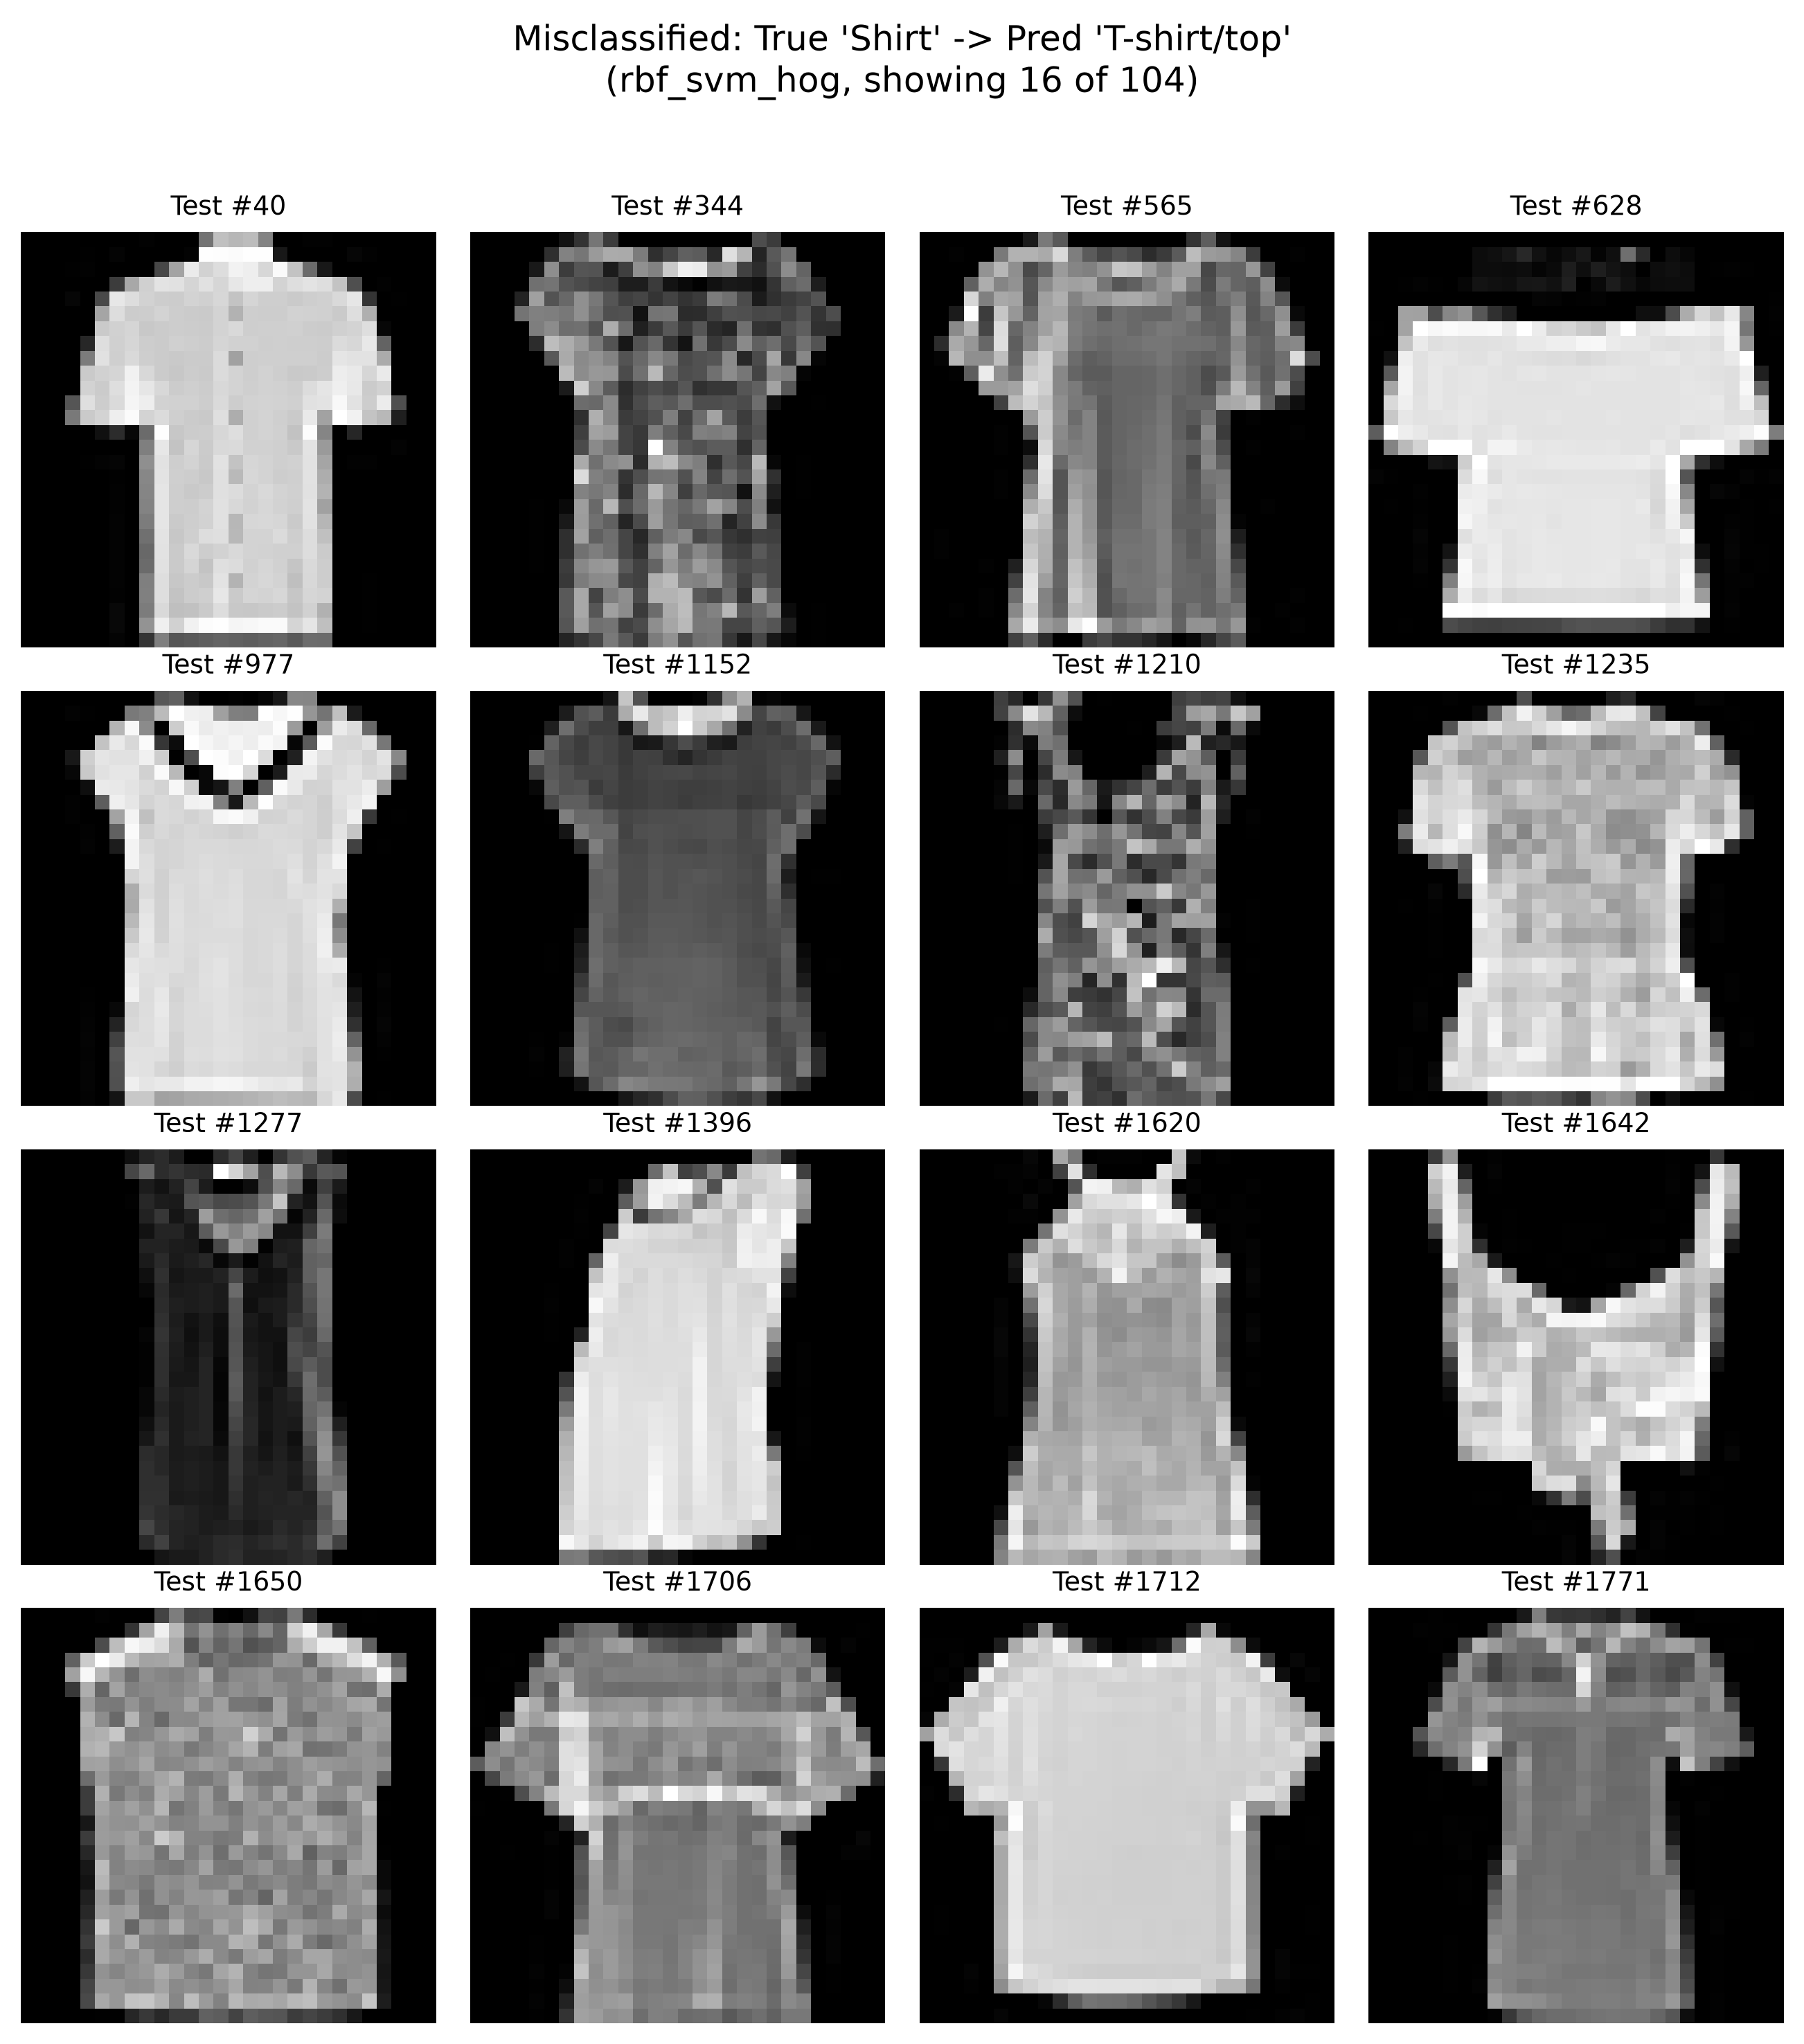
\includegraphics[width=0.9\linewidth]{errors_misclassified_shirt_vs_t-shirt_top.png}
  \caption{The first 16 test images of class Shirt predicted as T-shirt/top by the selected model (104 in total).}
  \label{fig:mis}
\end{figure}

\textbf{Do the two best models make the same mistakes?} Comparing the saved predictions of the RBF SVM on HOG and on
pixels: 8,593 images are right for both, 515 wrong for both, 377 wrong only with HOG and 515 wrong only with pixels. HOG
therefore fixes 138 more images than it breaks, exactly the 1.38-point test gap. Of the 515 shared mistakes, 391 have the
\emph{same} wrong label and 397 are upper-body garments. When two models built on very different features make the same
mistake, the image itself is likely ambiguous rather than the model unlucky.

% -------------------------------------------------------------------------------------
\section{Discussion and Limitations}
\begin{itemize}
  \item \textbf{Grid edges.} Three models selected a value at the edge of their grid; wider grids might add a little
        accuracy. We kept the planned grids to avoid extra test evaluations.
  \item \textbf{Optimistic validation.} Validation accuracy is above test accuracy for all ten trained models (by
        0.02--2.05 points), as expected when the best of several settings is selected on validation~\cite{cawley2010overfitting}.
        The ranking is unchanged, and the untouched test score is what we report.
  \item \textbf{Timing.} Timings come from two laptops (Apple M3 and M3 Pro) and two Logistic Regression timings are
        excluded, so only large speed gaps (10$\times$ or more) should be read as firm.
  \item \textbf{Cross-validation} was run on a 10,000-image subset for time reasons, so it measures stability, not final
        accuracy.
\end{itemize}

% -------------------------------------------------------------------------------------
\section{Conclusion and Future Work}
On Fashion-MNIST, a carefully tuned classical pipeline reaches 91.08\% test accuracy with an RBF SVM on HOG features,
chosen without ever using the test set for a decision. HOG features are the single biggest help for linear models, but
not for trees or nearest neighbours, and the most accurate model is also by far the slowest. The remaining errors are
concentrated in four upper-body garments whose distinguishing details (collars, buttons, cuffs) occupy only a few pixels
and are not captured well by fixed edge histograms.

In Phase 2 we will train a small convolutional network on the \emph{same} split and score it with the \emph{same}
evaluation code, so it drops straight into Table~\ref{tab:results}. Our hypothesis is that learned local filters can pick
up those small details and beat 91.08\%, mainly by reducing the Shirt, T-shirt/top, Pullover and Coat confusions.

\textbf{Reproducibility.} Code, the committed split, all result files, figures and a decision log with the reasoning
behind every choice are available at
\url{https://github.com/rajdeep-2004/fashion-image-classification-benchmark}. A fresh clone regenerates every result in
under two minutes.

% -------------------------------------------------------------------------------------
\begin{thebibliography}{99}

\bibitem{xiao2017fashion}
H.~Xiao, K.~Rasul, and R.~Vollgraf, ``Fashion-MNIST: a novel image dataset for benchmarking machine learning
algorithms,'' \emph{arXiv preprint arXiv:1708.07747}, 2017.

\bibitem{dalal2005histograms}
N.~Dalal and B.~Triggs, ``Histograms of oriented gradients for human detection,'' in \emph{Proc. IEEE Conf. Computer
Vision and Pattern Recognition (CVPR)}, 2005, pp.~886--893.

\bibitem{cortes1995support}
C.~Cortes and V.~Vapnik, ``Support-vector networks,'' \emph{Machine Learning}, vol.~20, no.~3, pp.~273--297, 1995.

\bibitem{breiman2001random}
L.~Breiman, ``Random forests,'' \emph{Machine Learning}, vol.~45, no.~1, pp.~5--32, 2001.

\bibitem{cover1967nearest}
T.~Cover and P.~Hart, ``Nearest neighbor pattern classification,'' \emph{IEEE Trans. Information Theory}, vol.~13,
no.~1, pp.~21--27, 1967.

\bibitem{fan2008liblinear}
R.-E.~Fan, K.-W.~Chang, C.-J.~Hsieh, X.-R.~Wang, and C.-J.~Lin, ``LIBLINEAR: A library for large linear
classification,'' \emph{Journal of Machine Learning Research}, vol.~9, pp.~1871--1874, 2008.

\bibitem{pedregosa2011scikit}
F.~Pedregosa \emph{et al.}, ``Scikit-learn: Machine learning in Python,'' \emph{Journal of Machine Learning Research},
vol.~12, pp.~2825--2830, 2011.

\bibitem{vanderwalt2014scikit}
S.~van der Walt \emph{et al.}, ``scikit-image: image processing in Python,'' \emph{PeerJ}, vol.~2, p.~e453, 2014.

\bibitem{vandermaaten2008tsne}
L.~van der Maaten and G.~Hinton, ``Visualizing data using t-SNE,'' \emph{Journal of Machine Learning Research}, vol.~9,
pp.~2579--2605, 2008.

\bibitem{kaufman2012leakage}
S.~Kaufman, S.~Rosset, C.~Perlich, and O.~Stitelman, ``Leakage in data mining: Formulation, detection, and avoidance,''
\emph{ACM Trans. Knowledge Discovery from Data}, vol.~6, no.~4, pp.~1--21, 2012.

\bibitem{cawley2010overfitting}
G.~C.~Cawley and N.~L.~C.~Talbot, ``On over-fitting in model selection and subsequent selection bias in performance
evaluation,'' \emph{Journal of Machine Learning Research}, vol.~11, pp.~2079--2107, 2010.

\end{thebibliography}

\end{document}
